
\documentclass[a4paper,12pt]{article}
\usepackage{graphicx}
\usepackage[table,xcdraw]{xcolor}
\usepackage{geometry}
\usepackage{float}
\usepackage[colorlinks=false, hidelinks]{hyperref}
\usepackage{fancyhdr}% For page numbering
\geometry{top=1in,bottom=1in,left=1in,right=1in}
\usepackage{listings}
\usepackage{xcolor}
\usepackage{hyperref}
\pagestyle{empty}


\begin{document}

\begin{center}
    \vspace{0.2cm}
    \textbf{\large{Lab Report: Sprint 1 Process}}\\
    \vspace{0.2cm}
    \textbf{Course Title: Software Engineering \& ISD Lab}\\
    \vspace{0.2cm}
    \textbf{Course Code: CSE-404}\\
    \vspace{0.2cm}
    \textbf{4\textsuperscript{th}Year 1\textsuperscript{st}Semester Examination 2023}\\
    \vspace{0.5cm}
    \textbf{Date of Submission: \today}\\

    \vspace{1.5cm}
    
\includegraphics[width=0.35\textwidth]{logo.png}\\ % Replace 'logo.png' with the correct path if you have the university logo image
    \vspace{1cm}

    \textbf{Submitted to}\\
    \vspace{0.2cm}
    \textbf{\href{https://juniv.edu/teachers/musfique.anwar}{Dr. Md Musfique Anwar}}\\
    {Professor}\\
    \vspace{0.2cm}
    \textbf{\href{https://juniv.edu/teachers/hkabir}{Dr. Md. Humayun Kabir}}\\
    {Professor}\\


    \vspace{1cm}

    \begin{table}[h!]
        \centering
        \arrayrulecolor{black}
        \begin{tabular}{|c|c|c|c|}
            \hline
            \rowcolor[HTML]{2F4F4F} % Changed header background color to dark slate gray
            {\color[HTML]{FFFFFF}\textbf{Sl}}& {\color[HTML]{FFFFFF}\textbf{Class Roll}}& {\color[HTML]{FFFFFF}\textbf{Exam Roll}}& {\color[HTML]{FFFFFF}\textbf{Name}}\\ \hline
            \rowcolor[HTML]{B0E0E6}
            \textbf{1}& \textbf{408} & \textbf{202220} & \textbf{Sudipta Singha} \\ \hline
       
        \end{tabular}
    \end{table}

    \vspace{1cm}

    Department of Computer Science and Engineering\\
    Jahangirnagar University\\
    Savar, Dhaka, Bangladesh\\
\end{center}

\newpage

\tableofcontents

\newpage
\pagestyle{fancy}
\fancyhf{}
\fancyfoot[C]{\thepage} % Page number in the center of the footer
\section{Introduction}
The purpose of this lab was to gain practical experience with the Agile Scrum development process by
conducting a Sprint. The Sprint aimed to deliver a working iteration of the project within a time-boxed
duration of one week. Key activities included project backlog preparation, sprint planning, daily scrum
meetings, and a sprint retrospective. This report documents my involvement in the Sprint, including meeting
outcomes, actions performed, and reflections on the process.
\newpage
\section{Meeting Summary}
Out Project is on Jahangirnagar University Medical Center Management System.To start the actual development
process
a team meeting was held.The main goal of the meeting is to establish the foundational elements of the Sprint. During the meeting, the following outcomes were achieved:
\begin{itemize}
    \item \textbf{Project Backlog Creation:}\\All identified tasks were added to the Trello project
        backlog.These backlogs are shown bellow.
        \begin{enumerate}
            \item Create Account
            \item Login
            \item See Information of Waiting Patients
            \item Reschedule Test Appointments
            \item Make Appointment for Visiting a Doctor and Lab Tests
            \item Dispense Medicines to Patients
            \item Post about Seasonal Disease
            \item View Ambulance Information
            \item Submit Test Report
            \item Collect Test Reports and Prescriptions
            \item Prescribe Patients
            \item Certify for Fundrise
            \item Update Stock Information
            \item Visit the Seasonal Disease Portal
        \end{enumerate}
    \item \textbf{Roles Assigned:}
        \begin{itemize}
            \item Product Owner: Hasan Al Mamun
            \item Scrum Master: Subarna Saha
            \item Scrum Members: 
                \begin{itemize}
                    \item \textbf{Sudipta Singha}
                    \item Fatima Binte Aziz
                    \item Shabrina Shahana
                    \item Saud Al Nahian

                \end{itemize}
        \end{itemize}

    \item \textbf{Sprint Backlog Agreement:}\\Tasks were selected and prioritized for Sprint 1 in consultation
        with the project owner.The tasks are also assigned to members. The Sprint 1 backlog which are decided are.
        \begin{enumerate}
            \item Create Account(\textbf{Sudipta Singha})
            \item Login(\textbf{Subarna Saha})
            \item See Information of Waiting Patients(\textbf{Subarna Saha})
            \item Reschedule Test Appointments(\textbf{Shabrina Shahana})
            \item Make Appointment for Visiting a Doctor and Lab Tests(\textbf{Fatima Binte Aziz})
            \item Dispense Medicines to Patients(\textbf{Sudipta Singha})
            \item Post about Seasonal Disease(\textbf{Hasan Al Mamun})
            \item View Ambulance Information(\textbf{Saud Al Nahian})

        \end{enumerate}
    \item \textbf{Git Branch Name Convention: }Everyone will start working on the project in a branch named
        \textbf{branch-feature-member\_name\_initials} (e.g., branch-log-in-ss).
    \item \textbf{Git Commit Message Convention: }The format of the git commit messages was decided.
    \item \textbf{Discord Integration: } The decision to create a discord channel in our projects discord server to
        facilitate seamless communication during sprint 1 was taken.
    \item \textbf{Sprint Goals Defined: }The team agreed on the primary objectives and deliverables for Sprint
        1.
\end{itemize}
\newpage
\section{Actions Performed}
\begin{itemize}
    \item \textbf{Trello Setup:}
        \begin{itemize}
            \item Created columns for "Project backlog" and "Sprint-1 backlog".
            \item Updated Trello with tasks and description. 
            \item Assigned tasks to team members.
        \end{itemize}
    \item \textbf{Discord Channel Creation:}
        \begin{itemize}
            \item A discord channel named sprint-1 was created.
        \end{itemize}
    \item \textbf{Toggl time tracking:}
        \begin{itemize}
            \item A toggle project was created for time tracking.
        \end{itemize}
\end{itemize}
\begin{figure}[H]
    \centering
    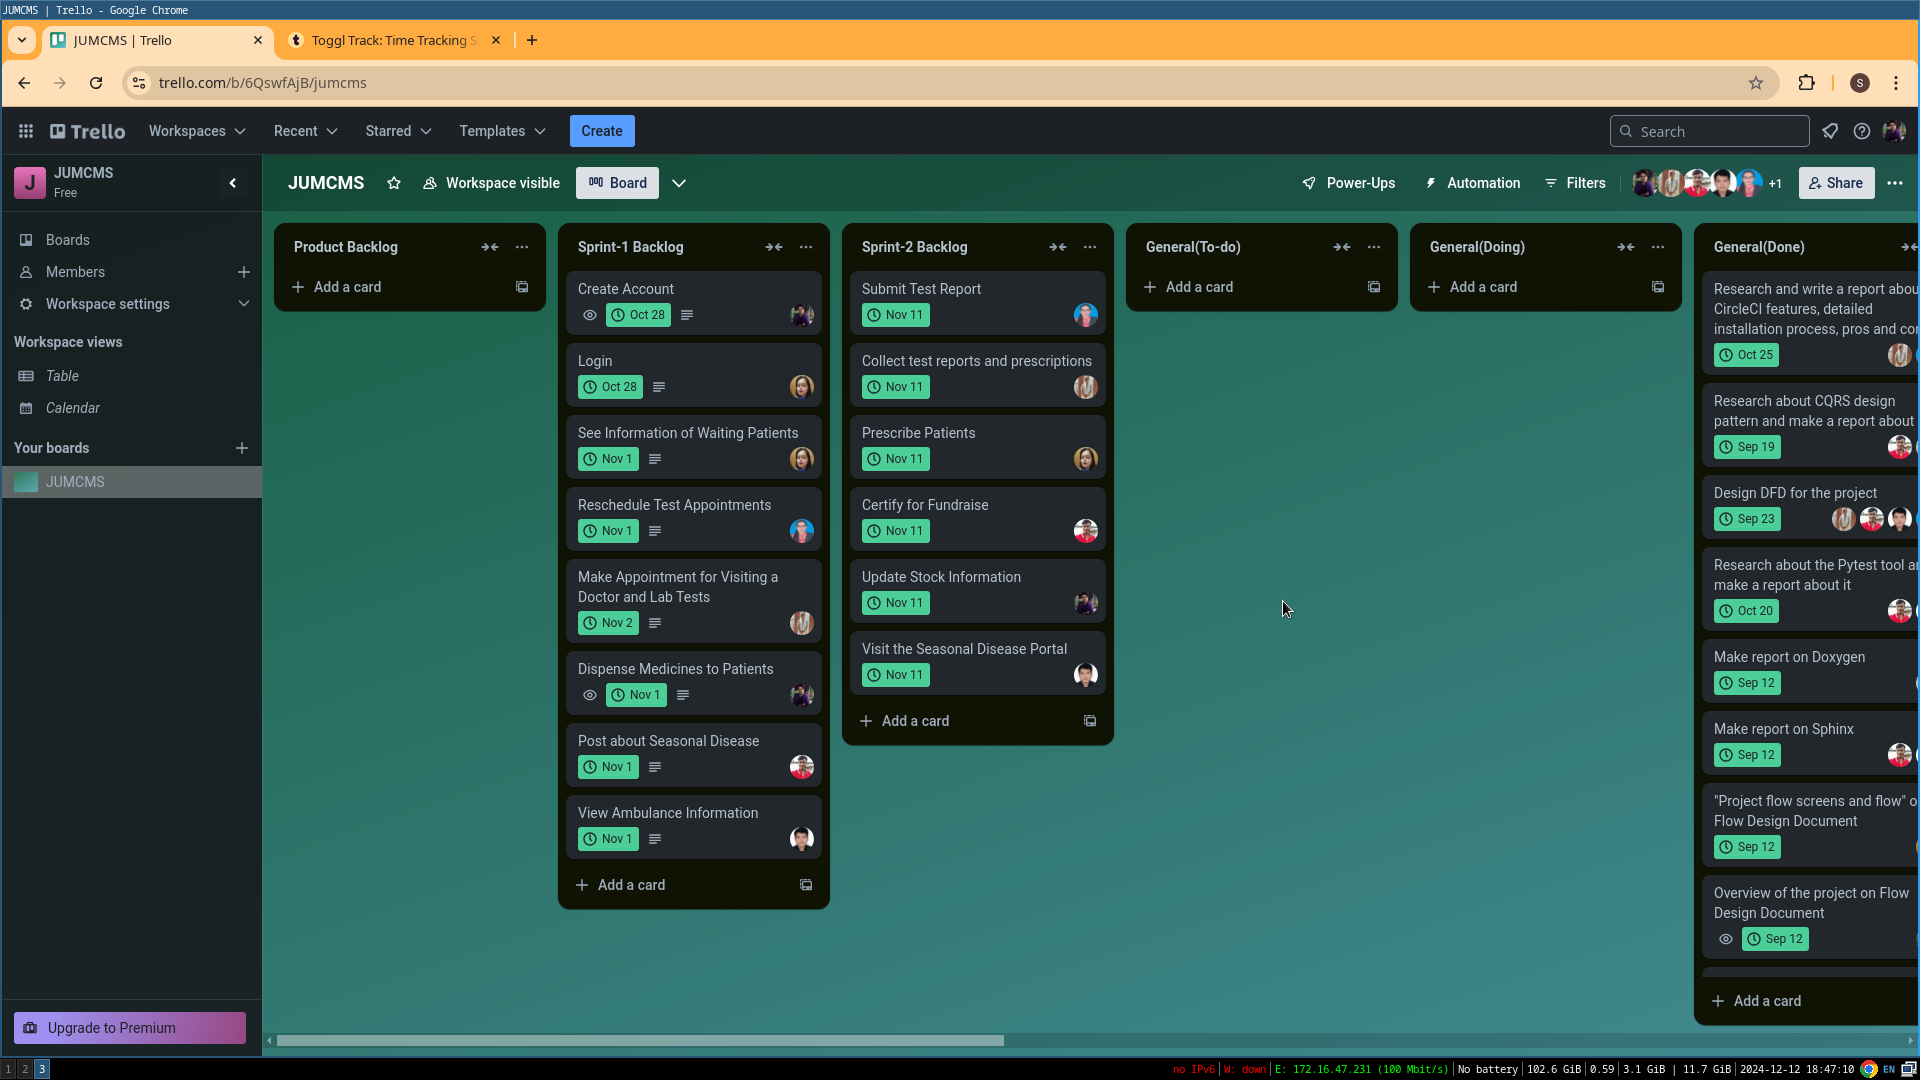
\includegraphics[width=\textwidth]{trello.png}
    \caption{Trello board}
\end{figure}

\begin{figure}[H]
    \centering
    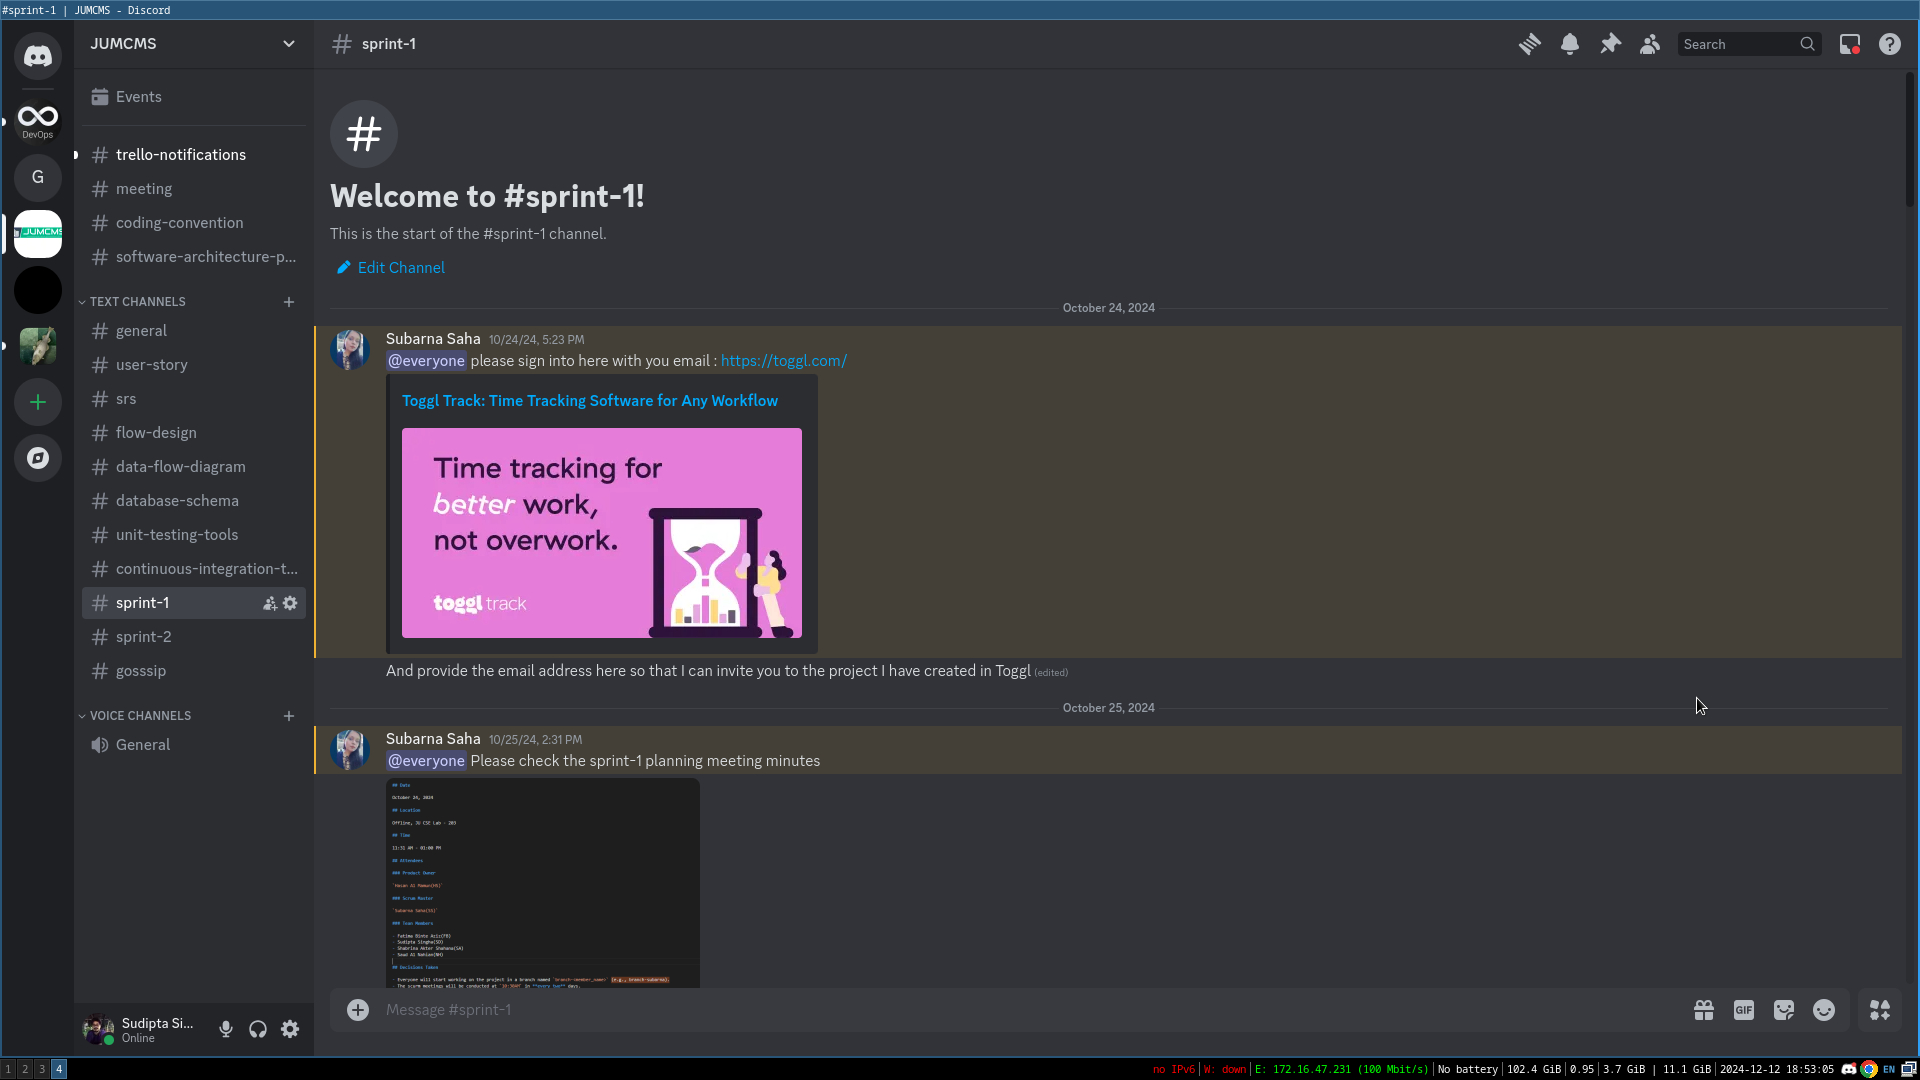
\includegraphics[width=\textwidth]{discord.png}
    \caption{Discord Channel}
\end{figure}

\begin{figure}[H]
    \centering
    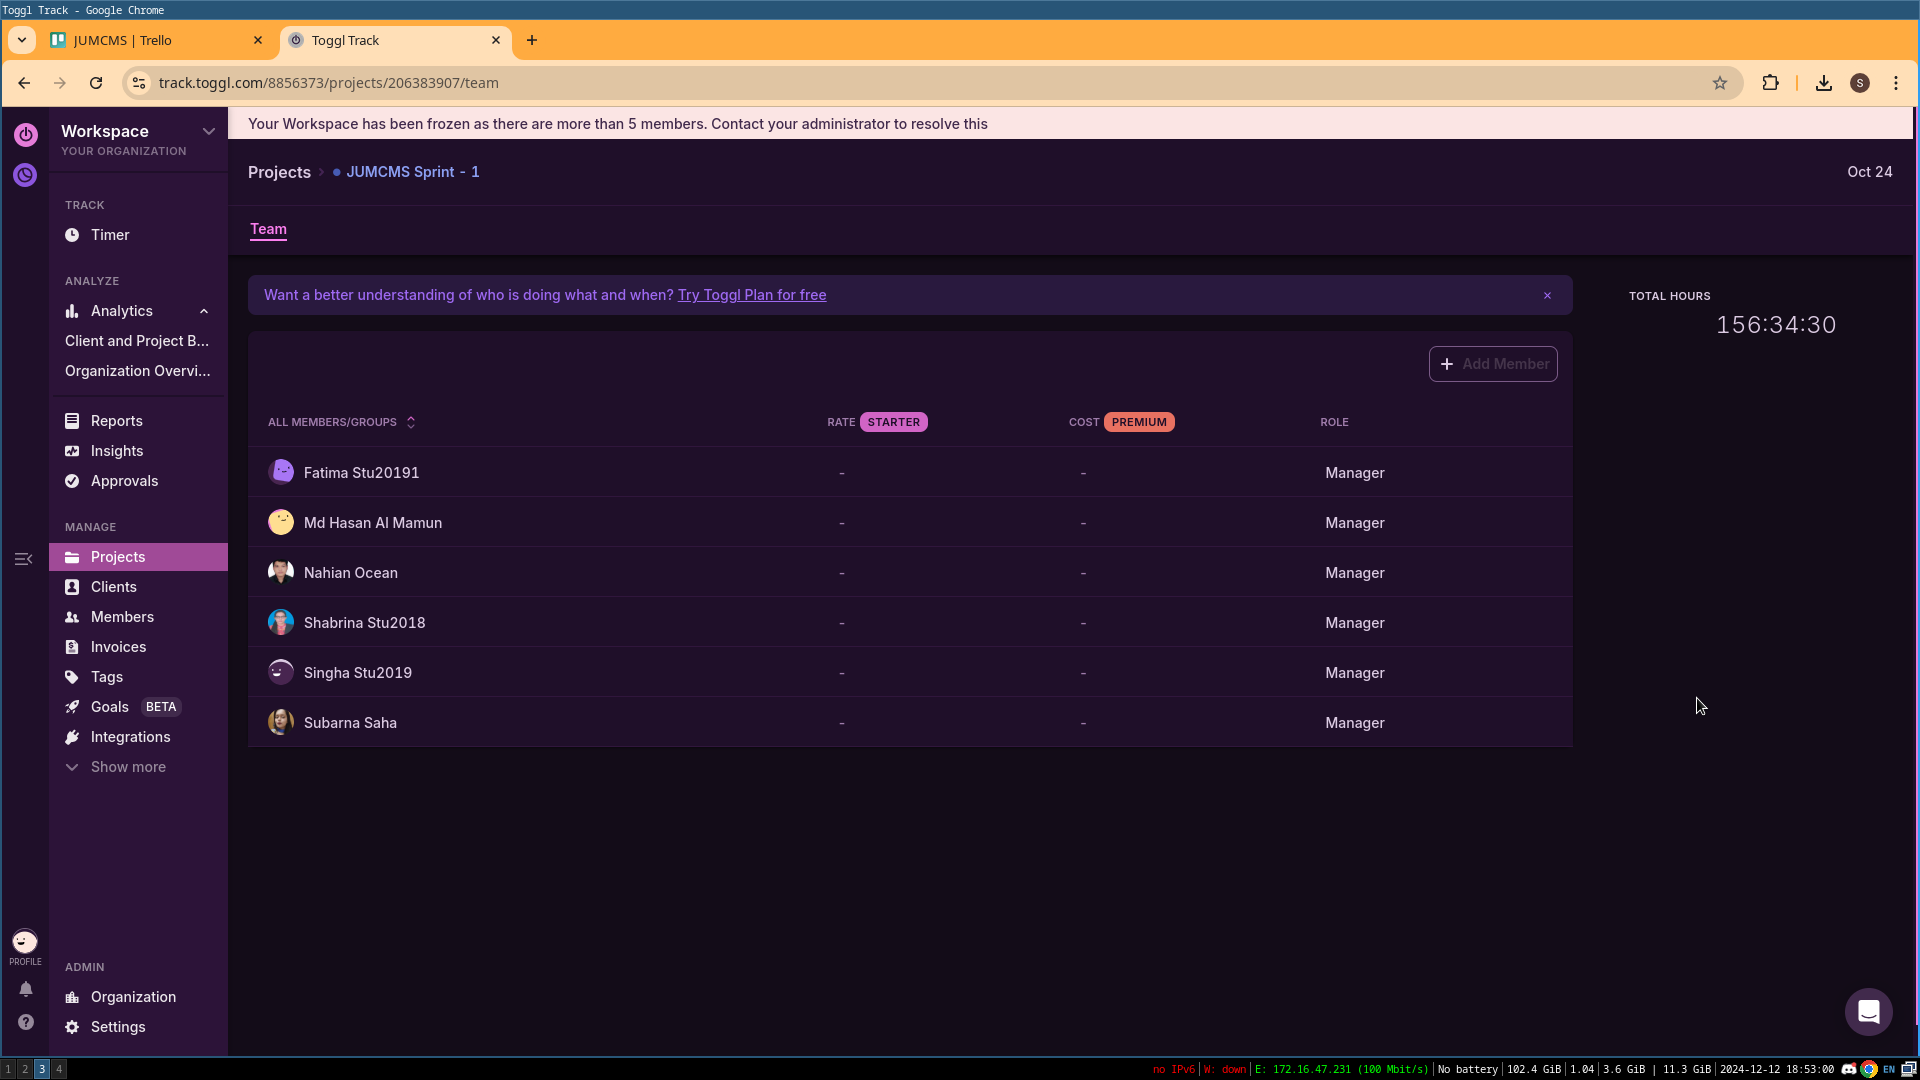
\includegraphics[width=\textwidth]{toggl.png}
    \caption{Toggl time tracking}
\end{figure}

\newpage
\section{Daily Scrum Meetings}
\subsection{Scrum Meeting 1}
My updates on progress are
\begin{itemize}
    \item Yesterday: Completed the coding for role-based registration of the JUMCMS.
    \item Today: Will prepare for unit tests for the Create account part.
    \item Impediments: None.
\end{itemize}
\textbf{\large{Screenshot of Git Activity}}
\begin{figure}[H]
    \centering
    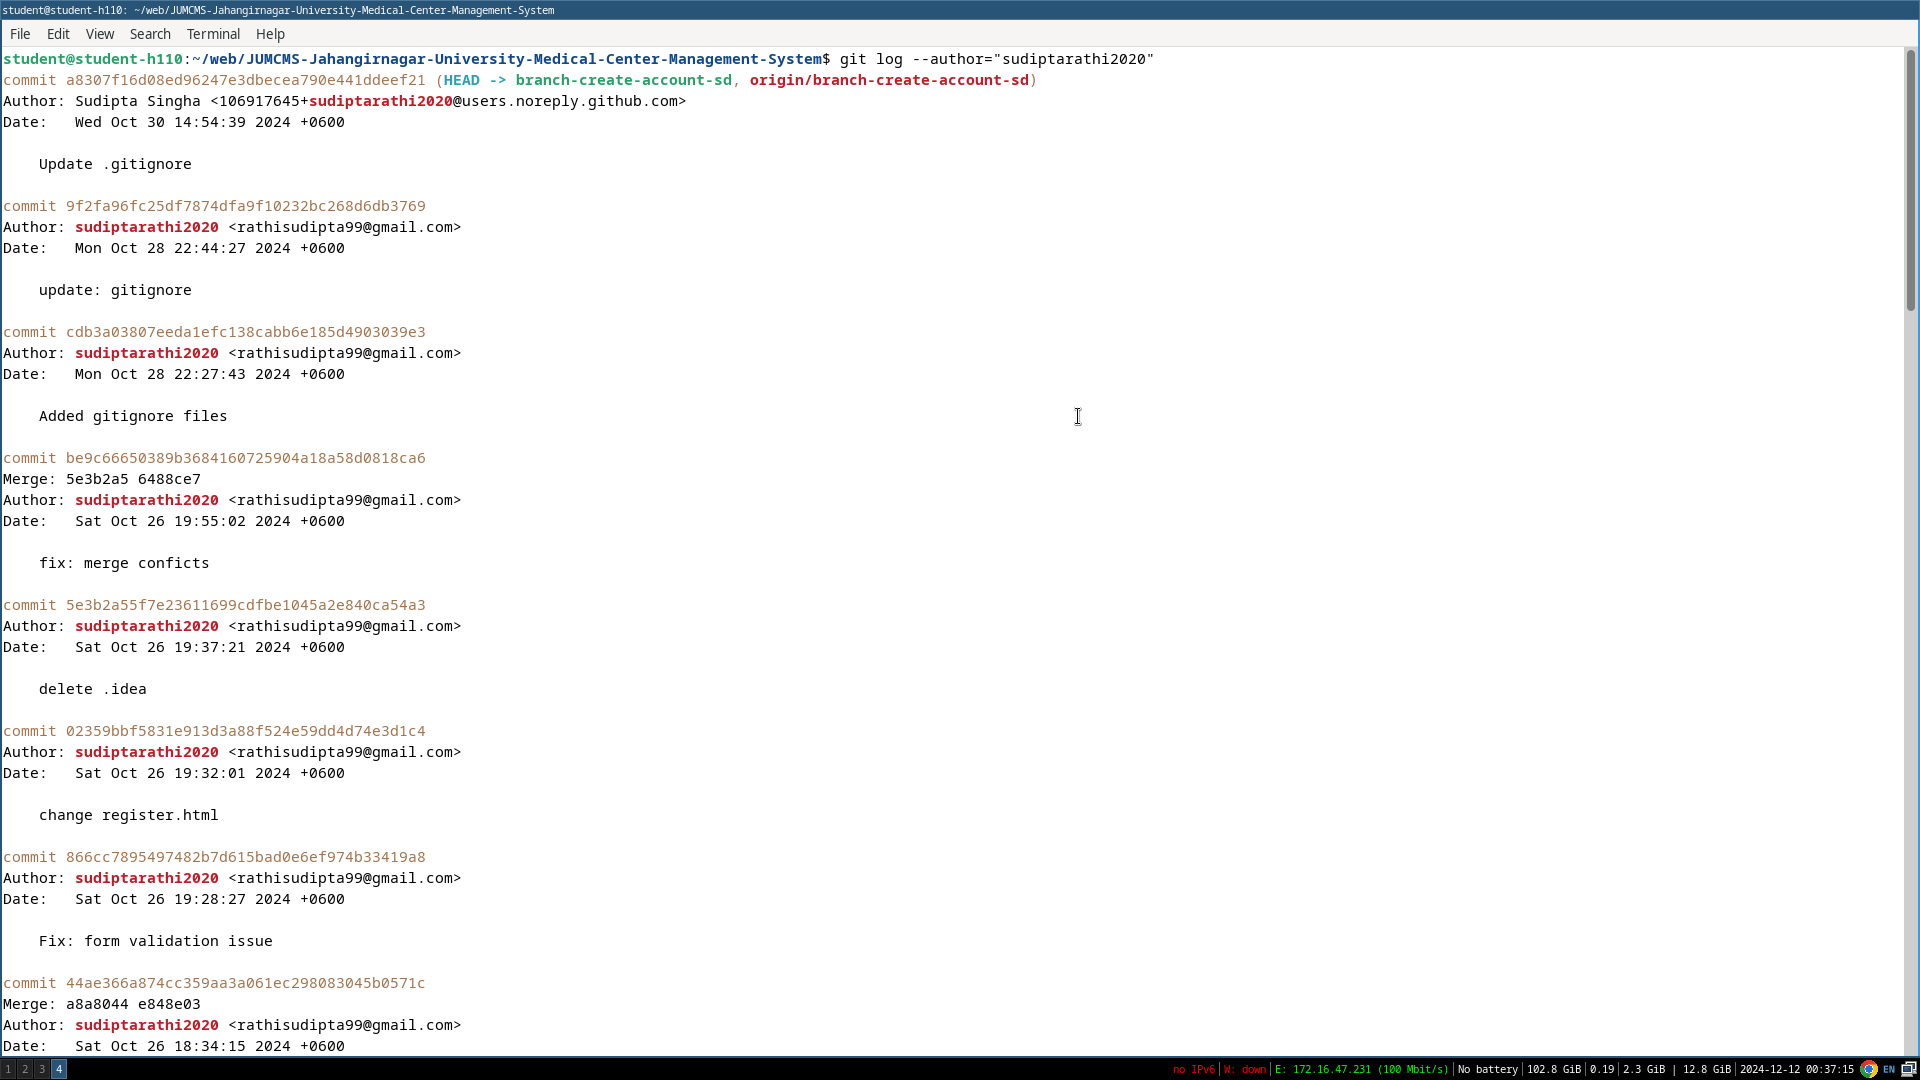
\includegraphics[width=\textwidth]{spr1meet11.png}
    \caption{My Git Log 1}
\end{figure}
\begin{figure}[H]
    \centering
    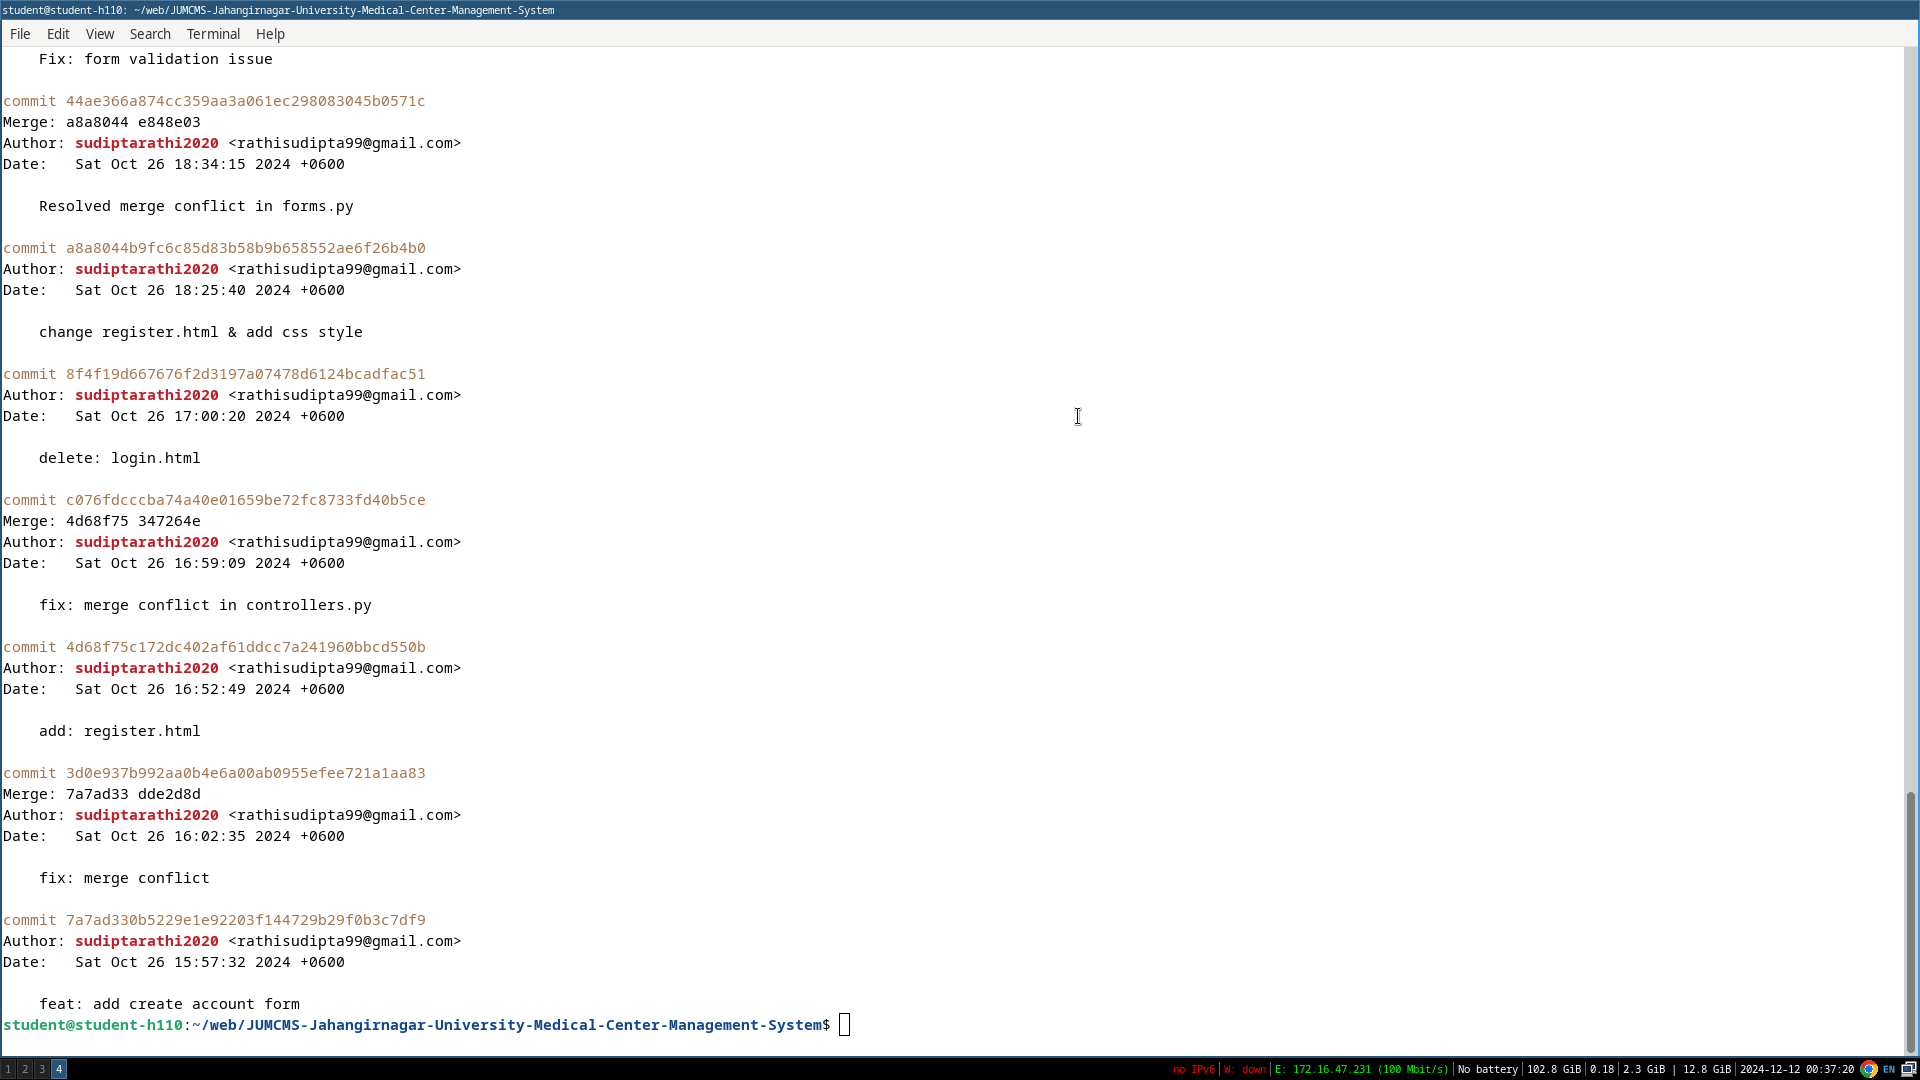
\includegraphics[width=\textwidth]{spr1meet12.png}
    \caption{My Git Log 2}
\end{figure}
\newpage
\subsection{Scrum Meeting 2}
After completing branch-create-account-sd's work, this branch is merged to branch-log-in-ss branch.
My updates on progress are
\begin{itemize}
    \item Yesterday: Completed unit tests for the Create account part.
    \item Today: Will start to design for Store-manager dashboard.
    \item Impediments: None.
\end{itemize}
\textbf{\large{Screenshot of Git Activity}}
\begin{figure}[H]
    \centering
    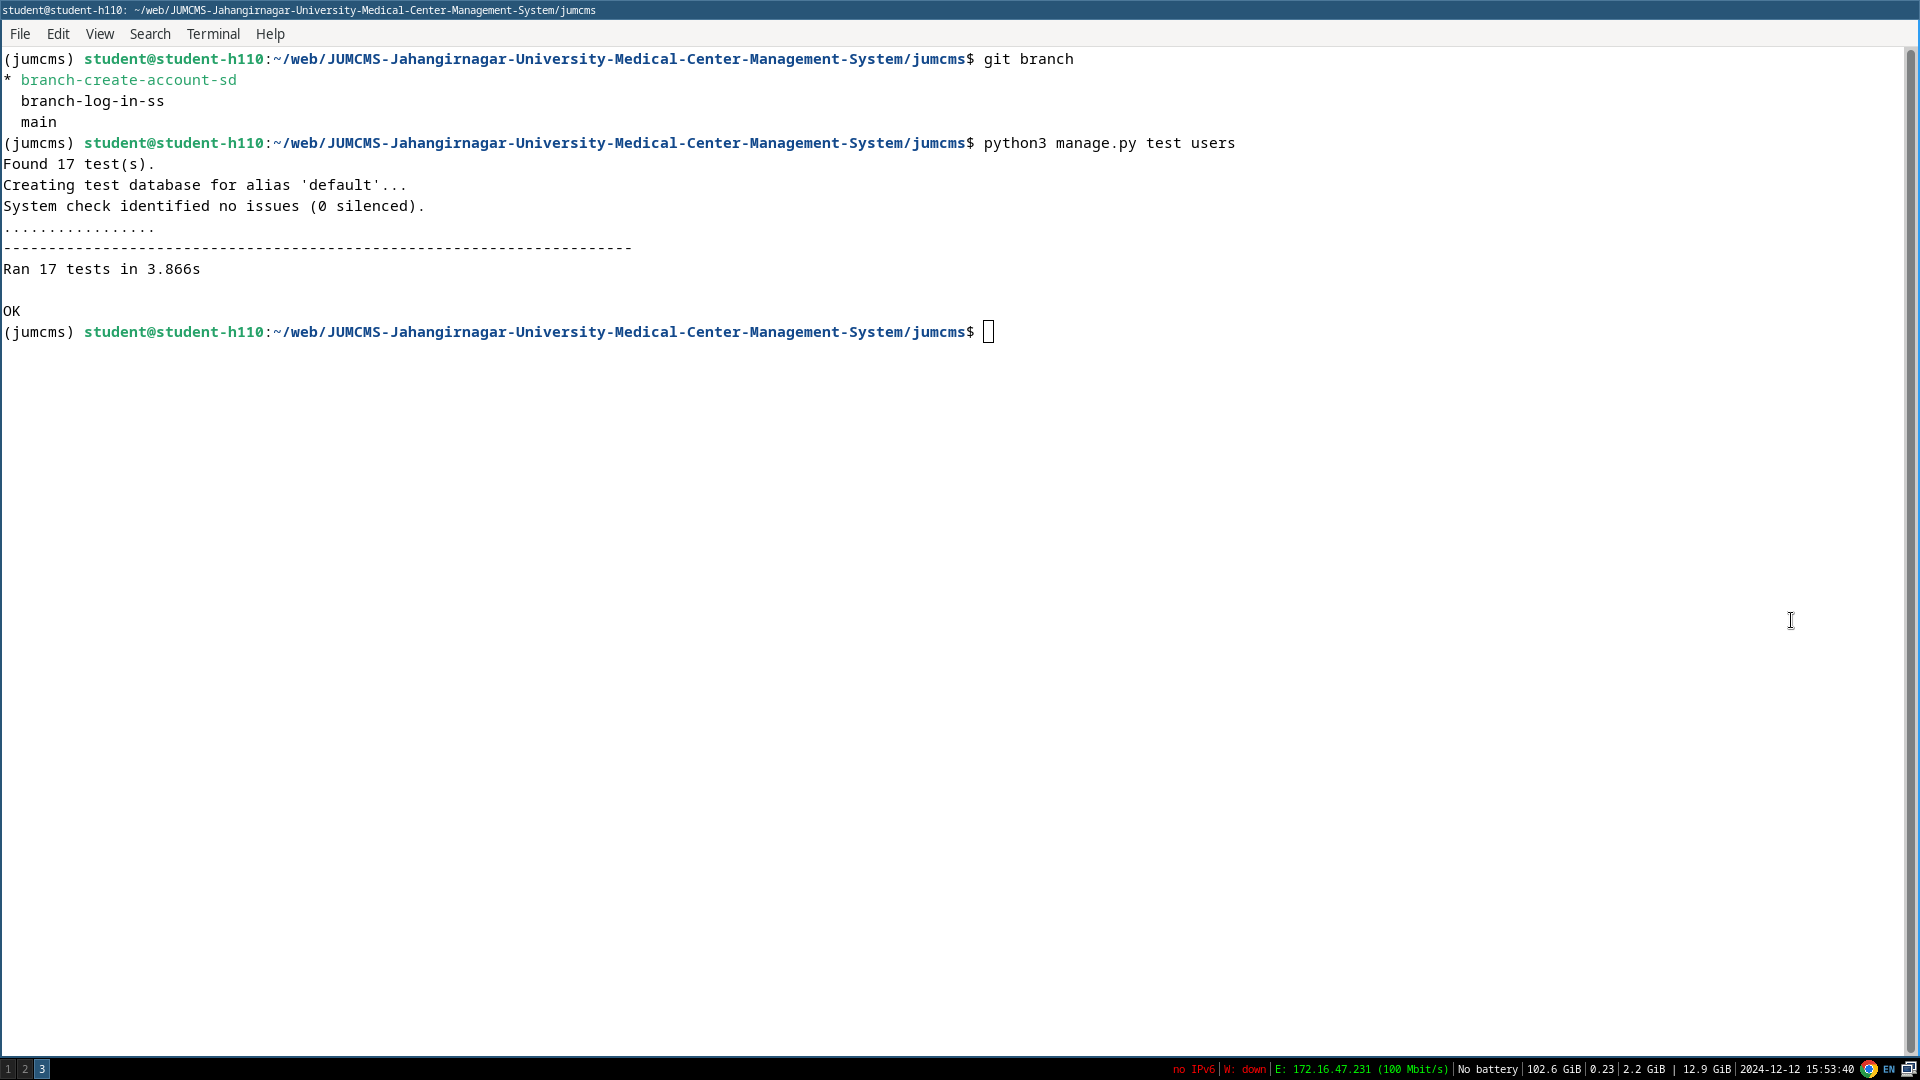
\includegraphics[width=\textwidth]{spr1meet21.png}
    \caption{Screenshot of Testing}
\end{figure}
\begin{figure}[H]
    \centering
    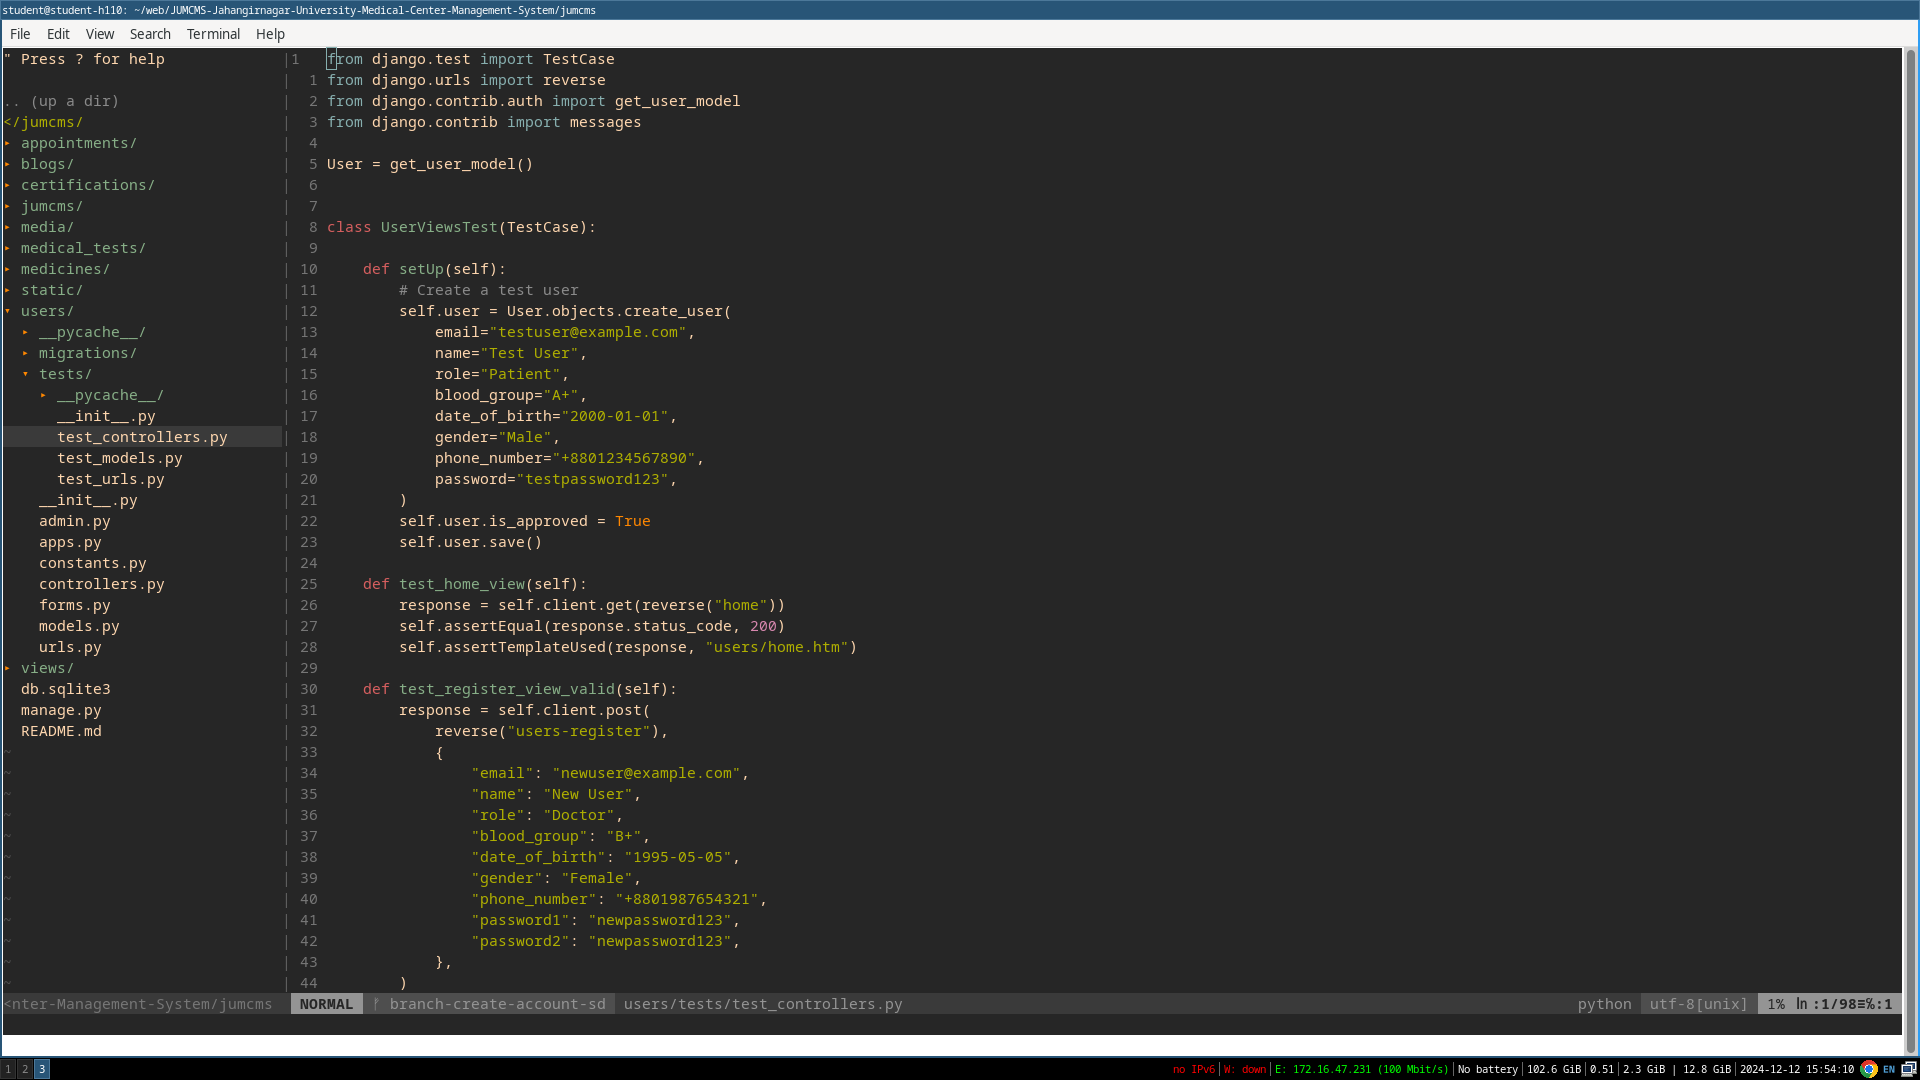
\includegraphics[width=\textwidth]{spr1meet22.png}
    \caption{Coding Testcase}
\end{figure}
\newpage
\subsection{Scrum Meeting 3}
I have been assigned two backlog for this sprint. They are create account and dispence medicine to patients.
Create account sprint backlog was completed in the last scrum meeting. In this week my updates on progress are
\begin{itemize}
    \item Yesterday: Implemented backend logic for the assigned task.
    \item Today: Will code for completing "Dispense medicine to patients" feature.
    \item Impediments: Facing challenges in URL routing.
\end{itemize}
The solution for my impediment is
\begin{itemize}
    \item Take help from \textbf{Subarna Saha} to solve the URL routing problem.
\end{itemize}
\textbf{\large{Screenshot of Git Activity}}
\begin{figure}[H]
    \centering
    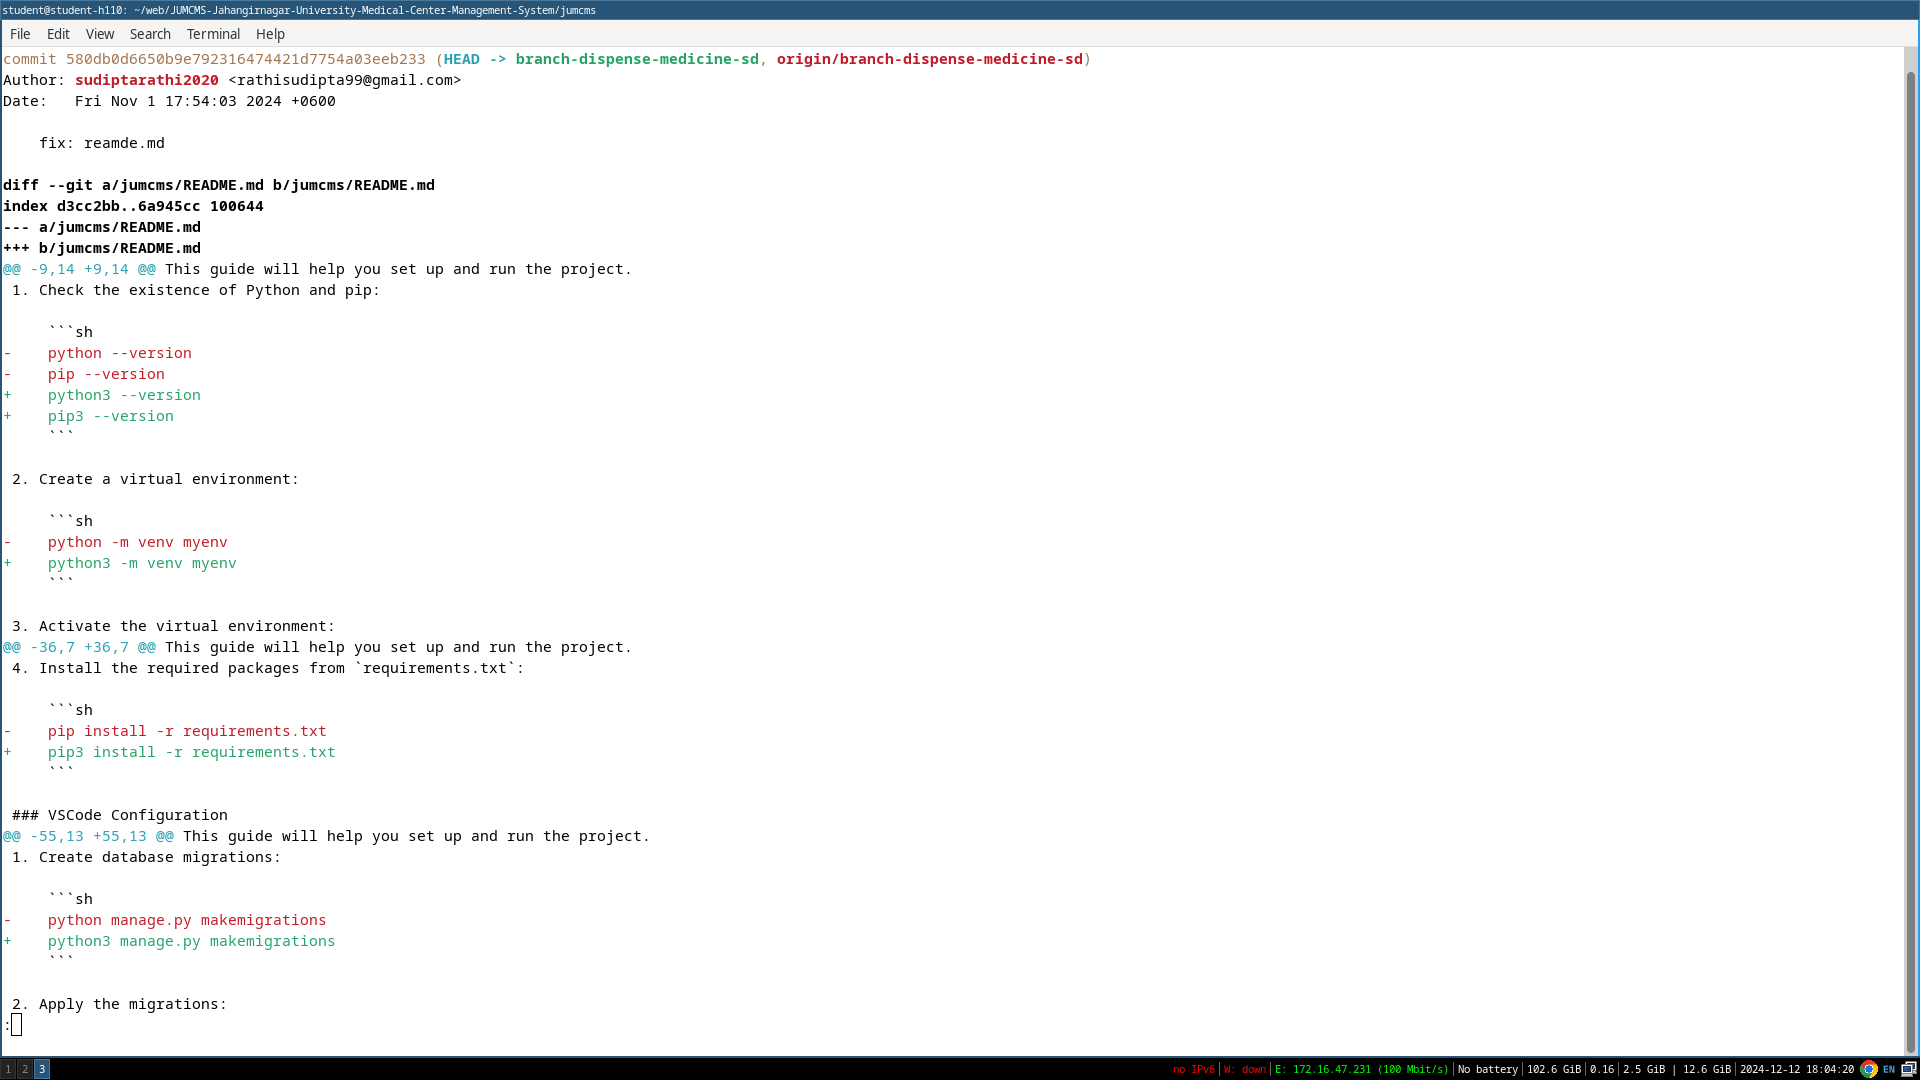
\includegraphics[width=\textwidth]{spr1meet31.png}
    \caption{git message: fix readme.md}
\end{figure}
\begin{figure}[H]
    \centering
    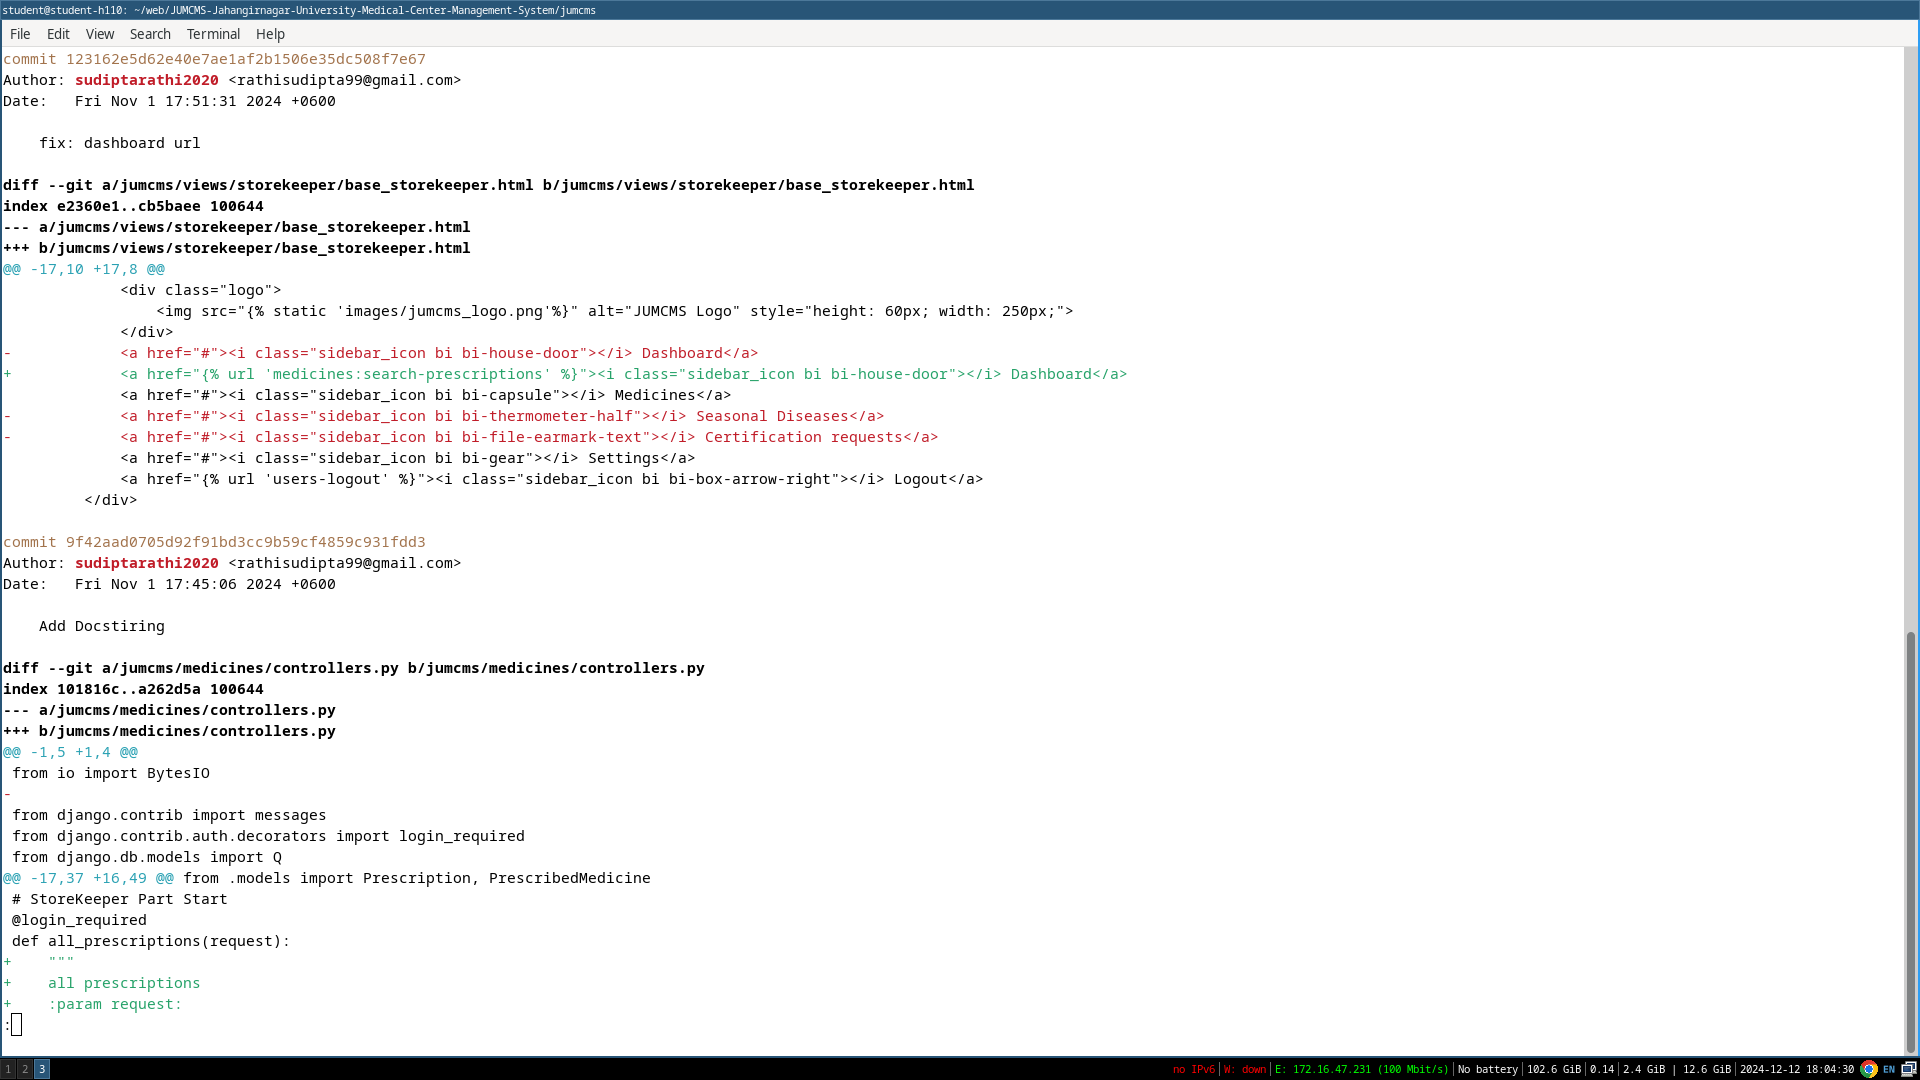
\includegraphics[width=\textwidth]{spr1meet32.png}
    \caption{git message: fix: dashboard url}
\end{figure}
\begin{figure}[H]
    \centering
    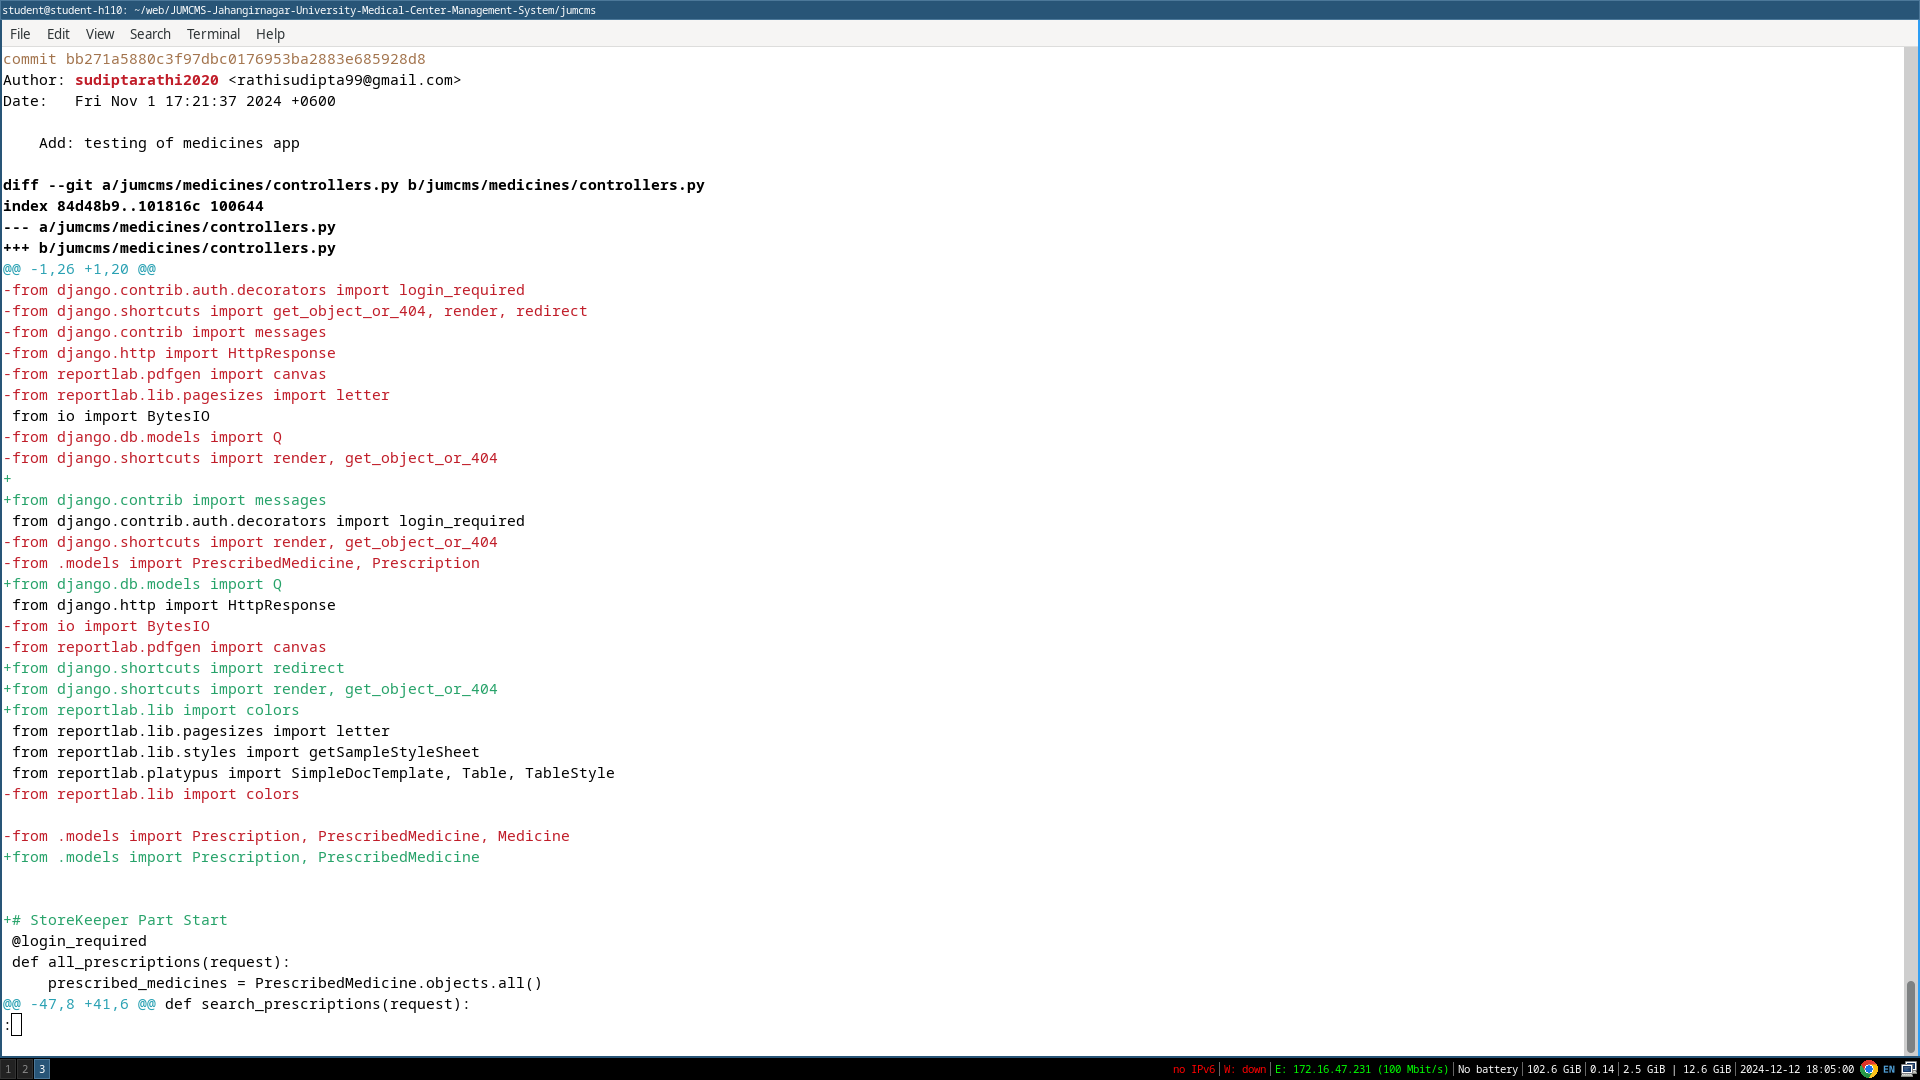
\includegraphics[width=\textwidth]{spr1meet33.png}
    \caption{git message: add:testing of medicine app}
\end{figure}


\begin{figure}[H]
    \centering
    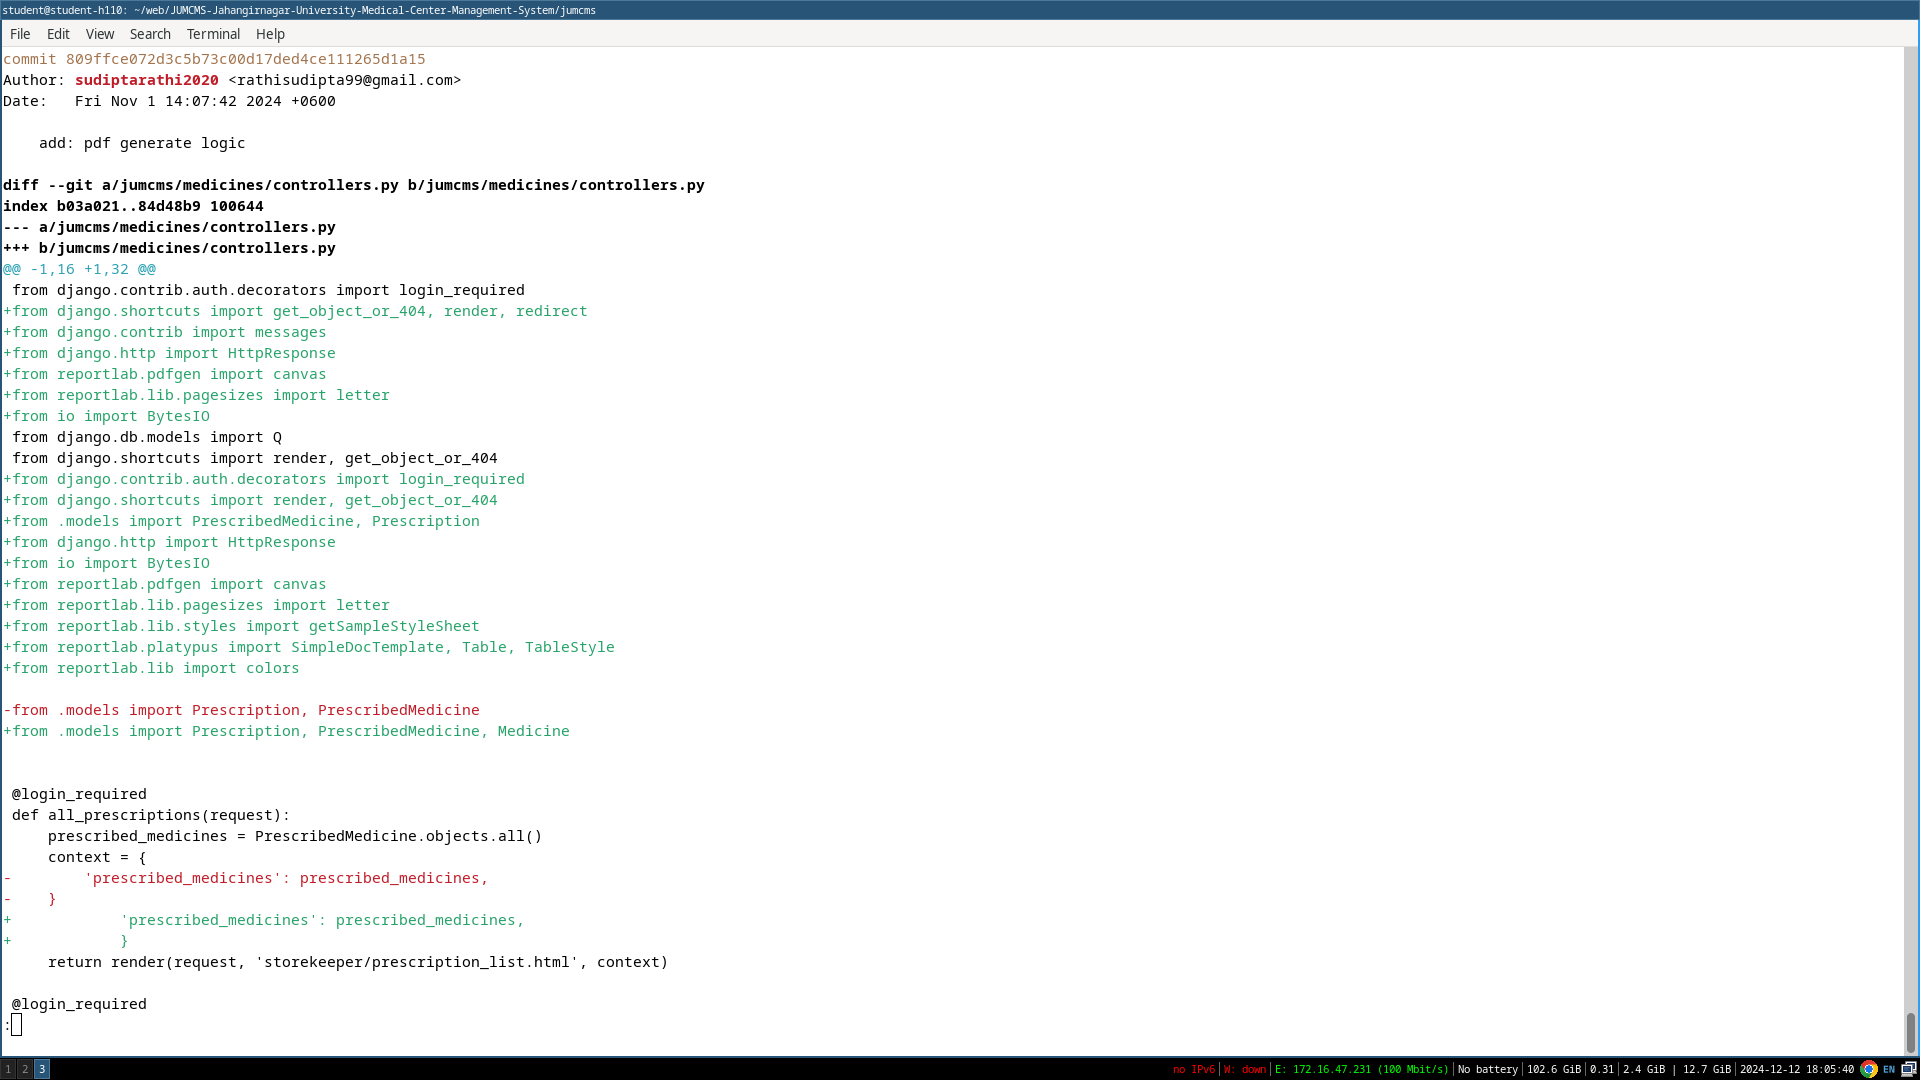
\includegraphics[width=\textwidth]{spr1meet34.png}
    \caption{git message: add: pdf generate logic}
\end{figure}


\begin{figure}[H]
    \centering
    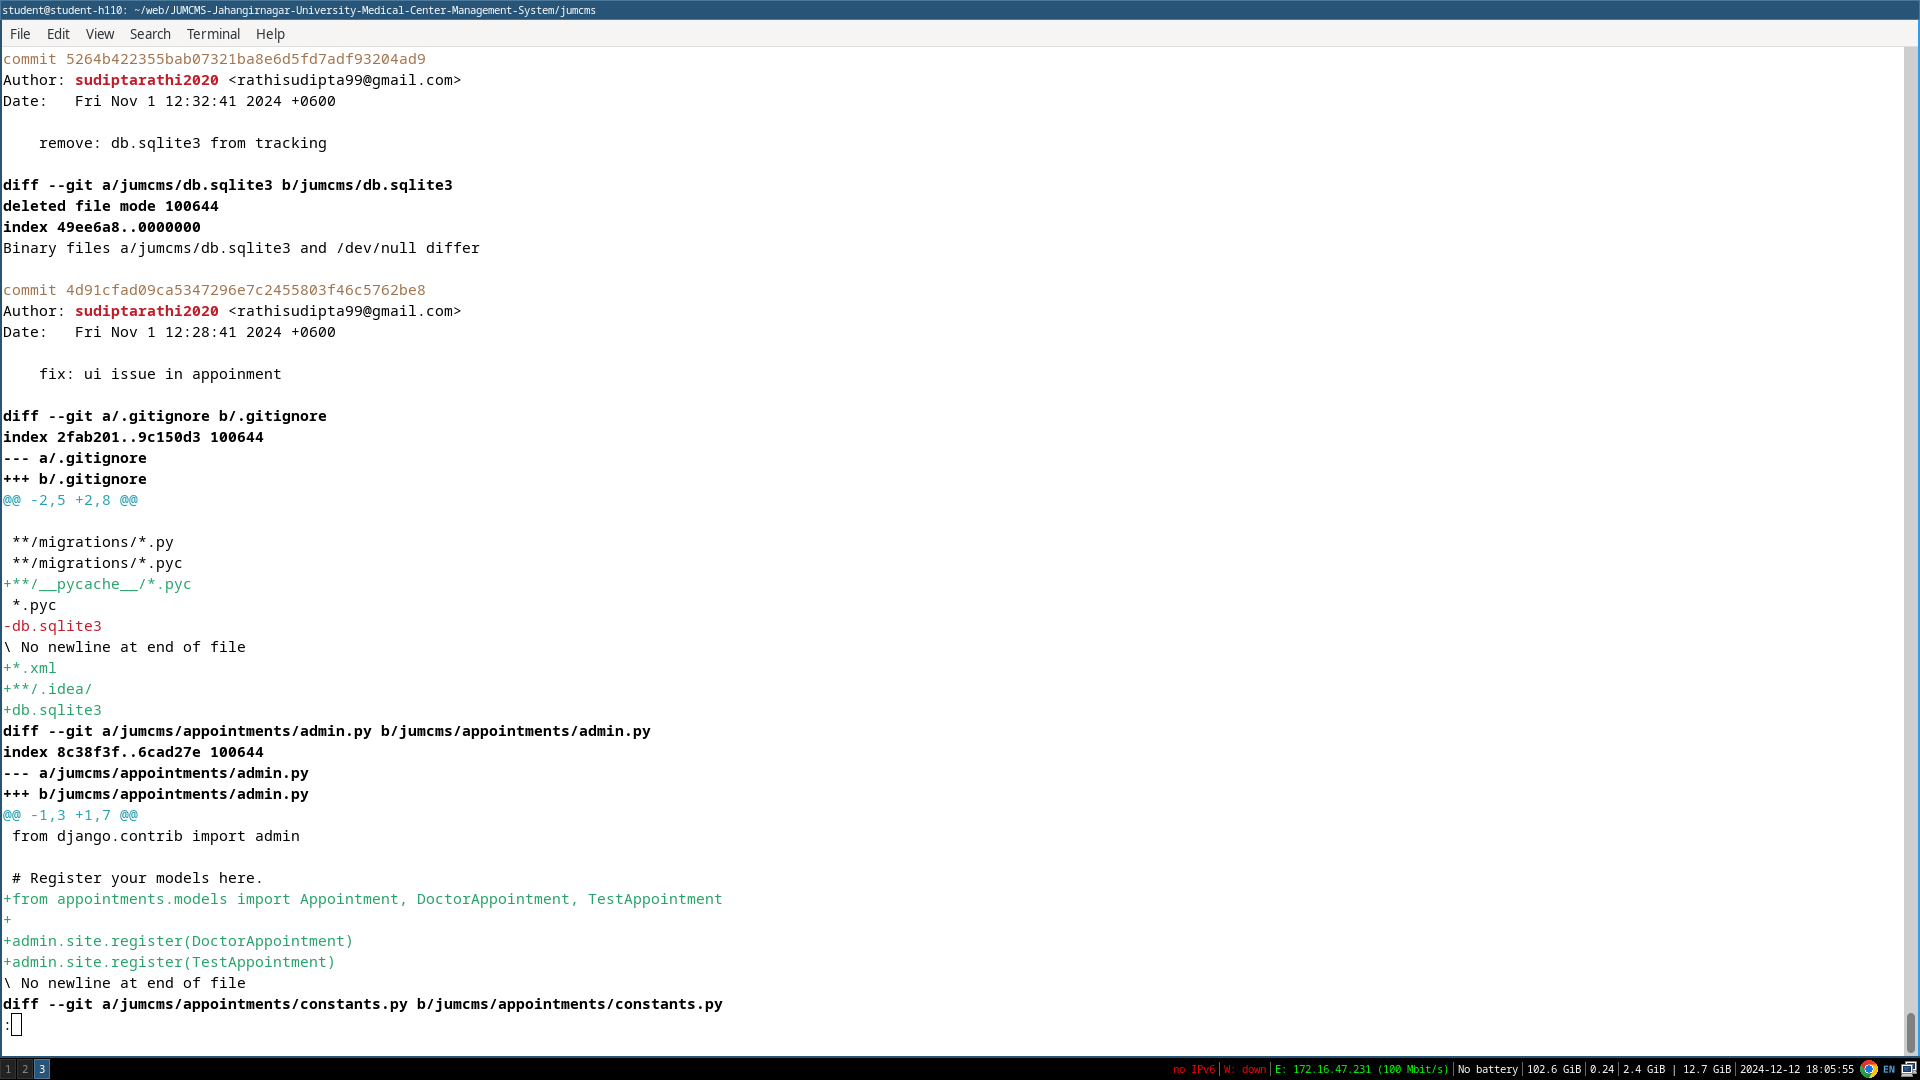
\includegraphics[width=\textwidth]{spr1meet35.png}
    \caption{git message: remove: db.sqlite3 from tracking \& fix ui issue in Appointment}
\end{figure}


\begin{figure}[H]
    \centering
    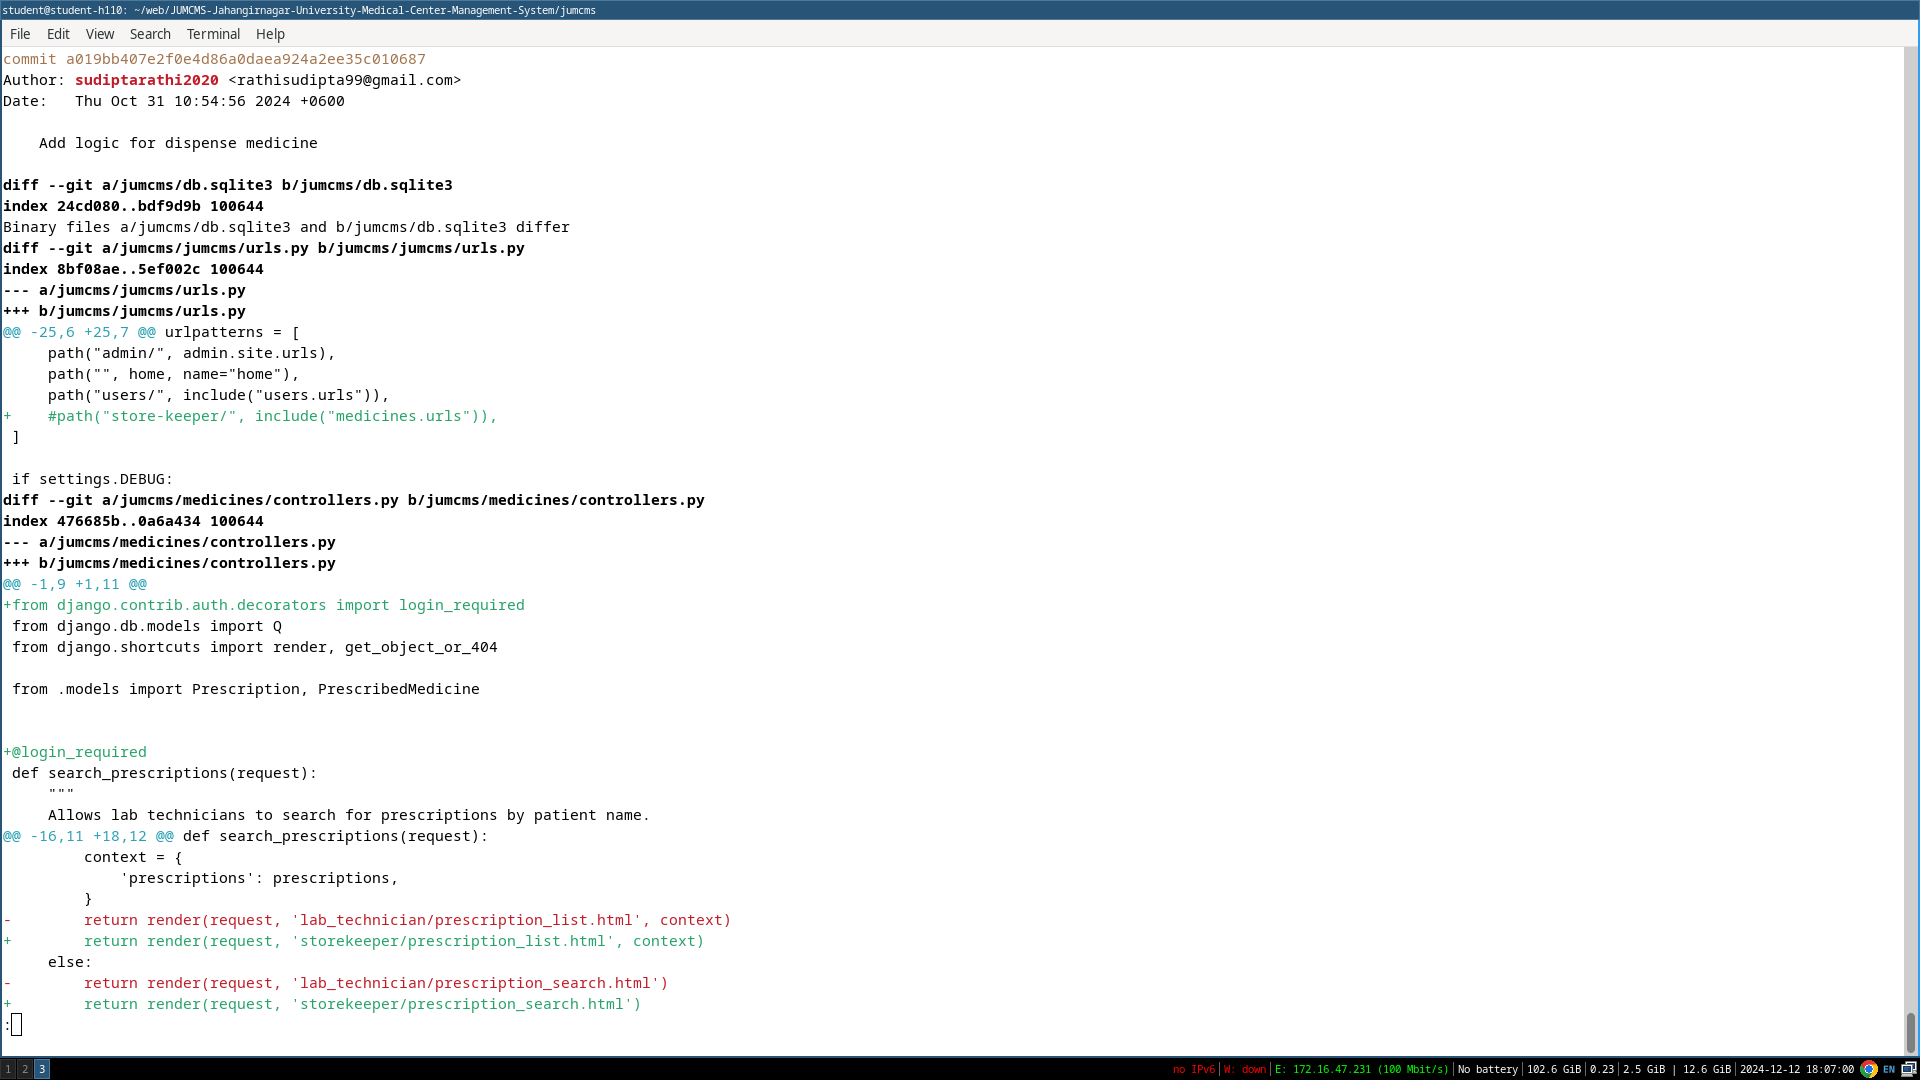
\includegraphics[width=\textwidth]{spr1meet36.png}
    \caption{git message:add: logic for dispense medicine}
\end{figure}


\begin{figure}[H]
    \centering
    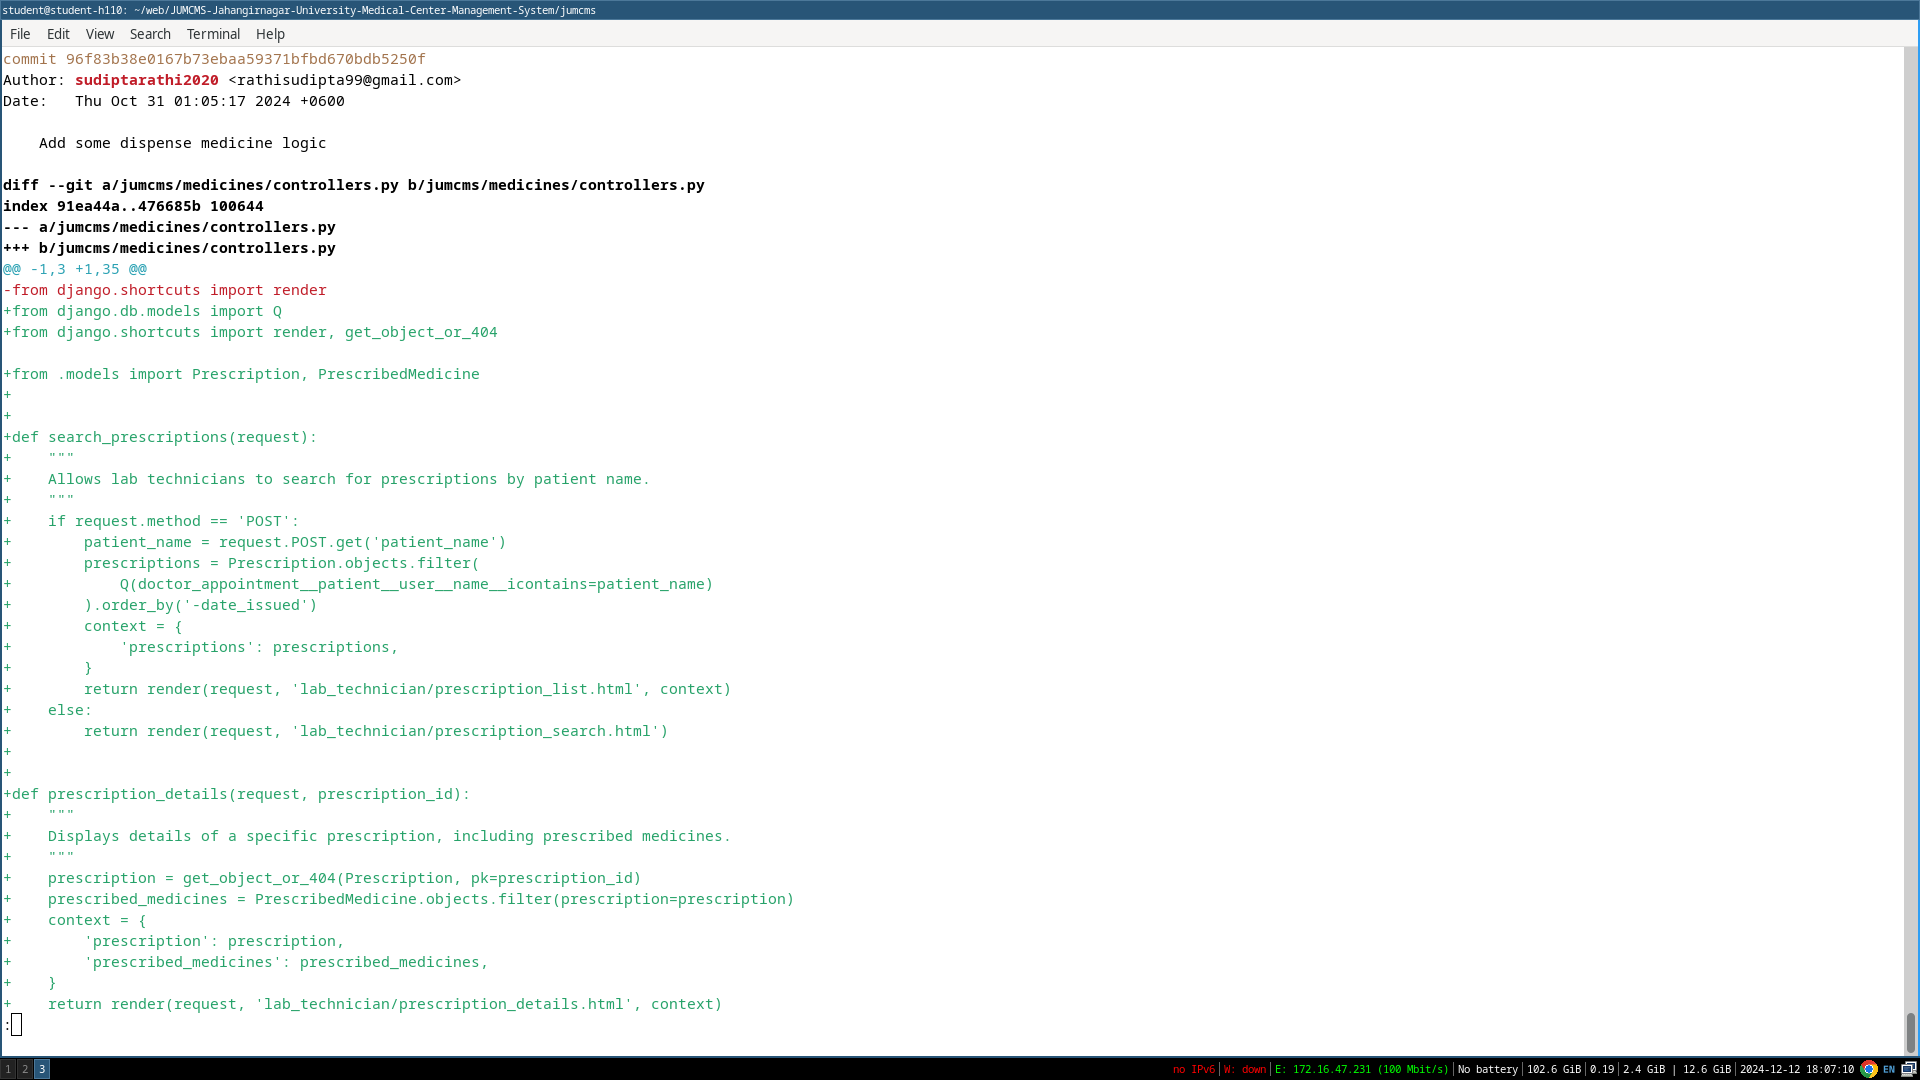
\includegraphics[width=\textwidth]{spr1meet37.png}
    \caption{}
\end{figure}


\begin{figure}[H]
    \centering
    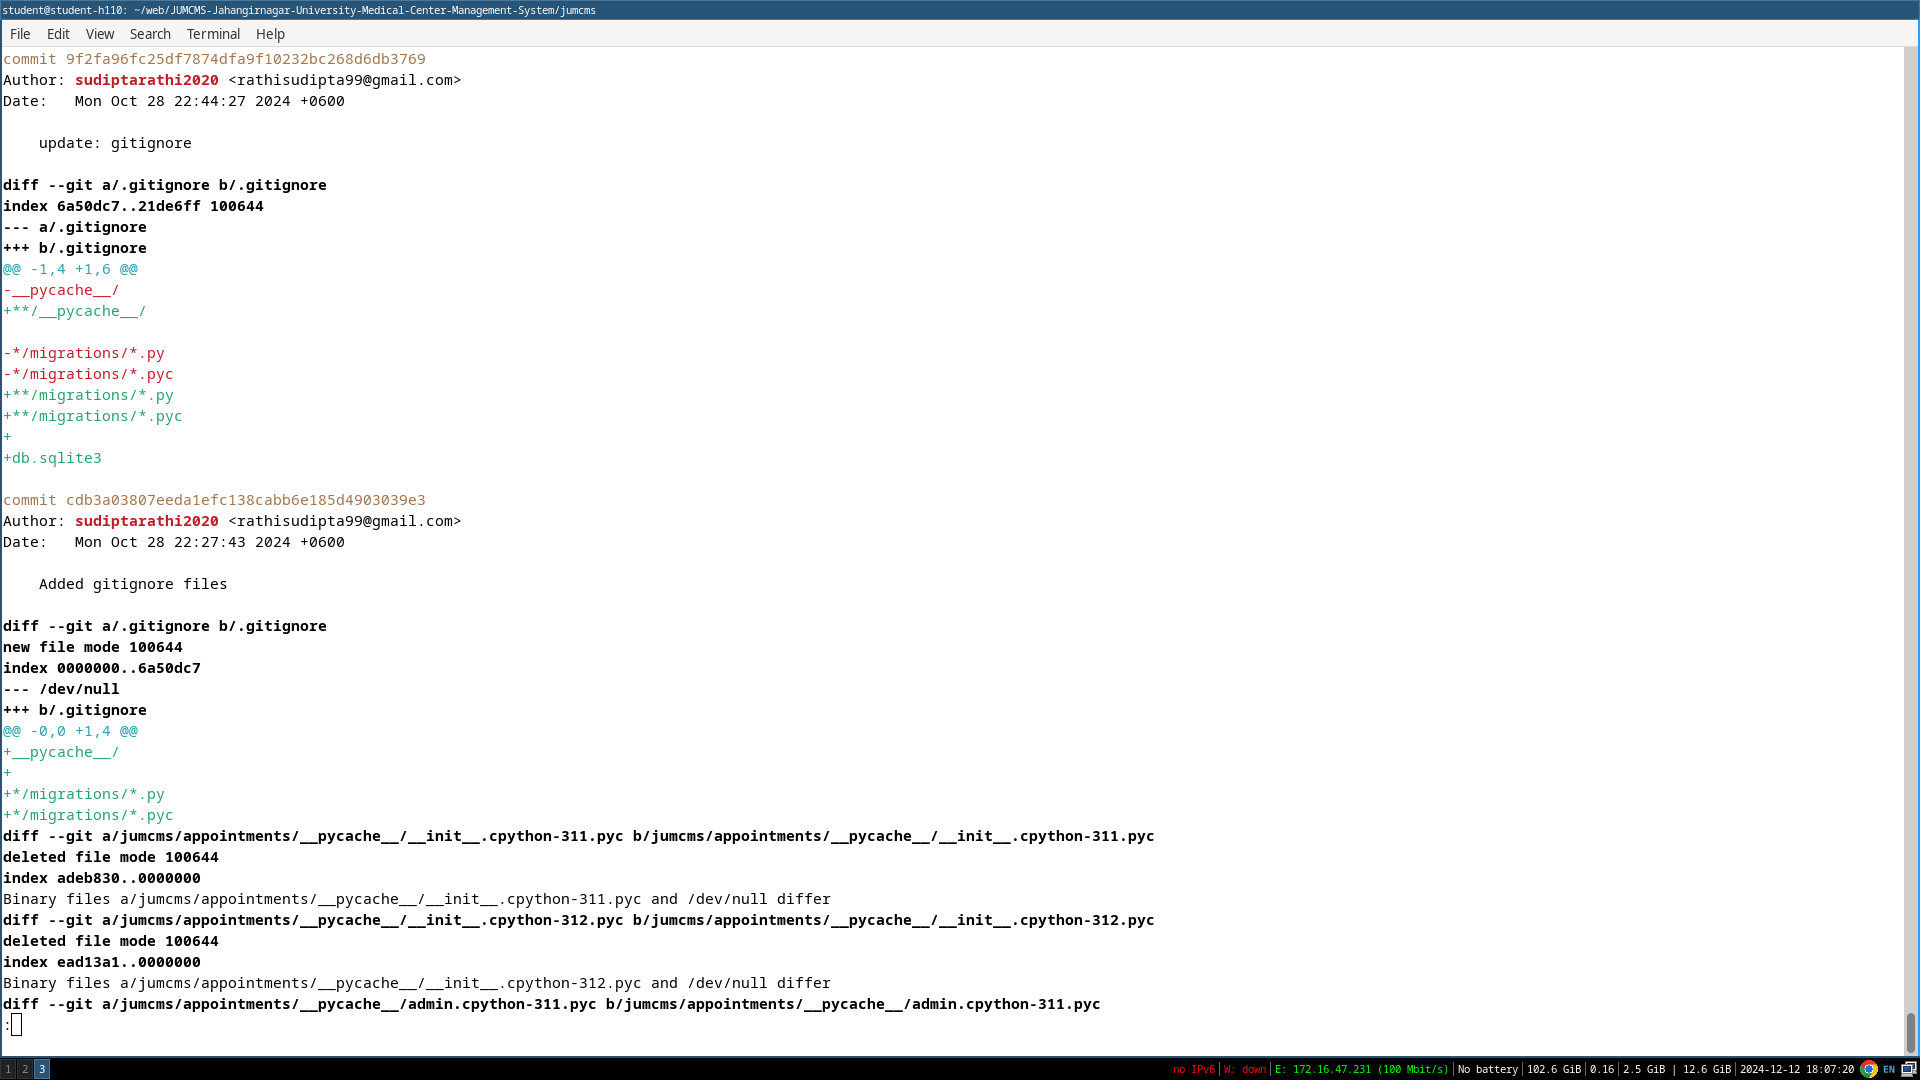
\includegraphics[width=\textwidth]{spr1meet38.png}
    \caption{git message: add dispense medicine logic}
\end{figure}

\begin{figure}[H]
    \centering
    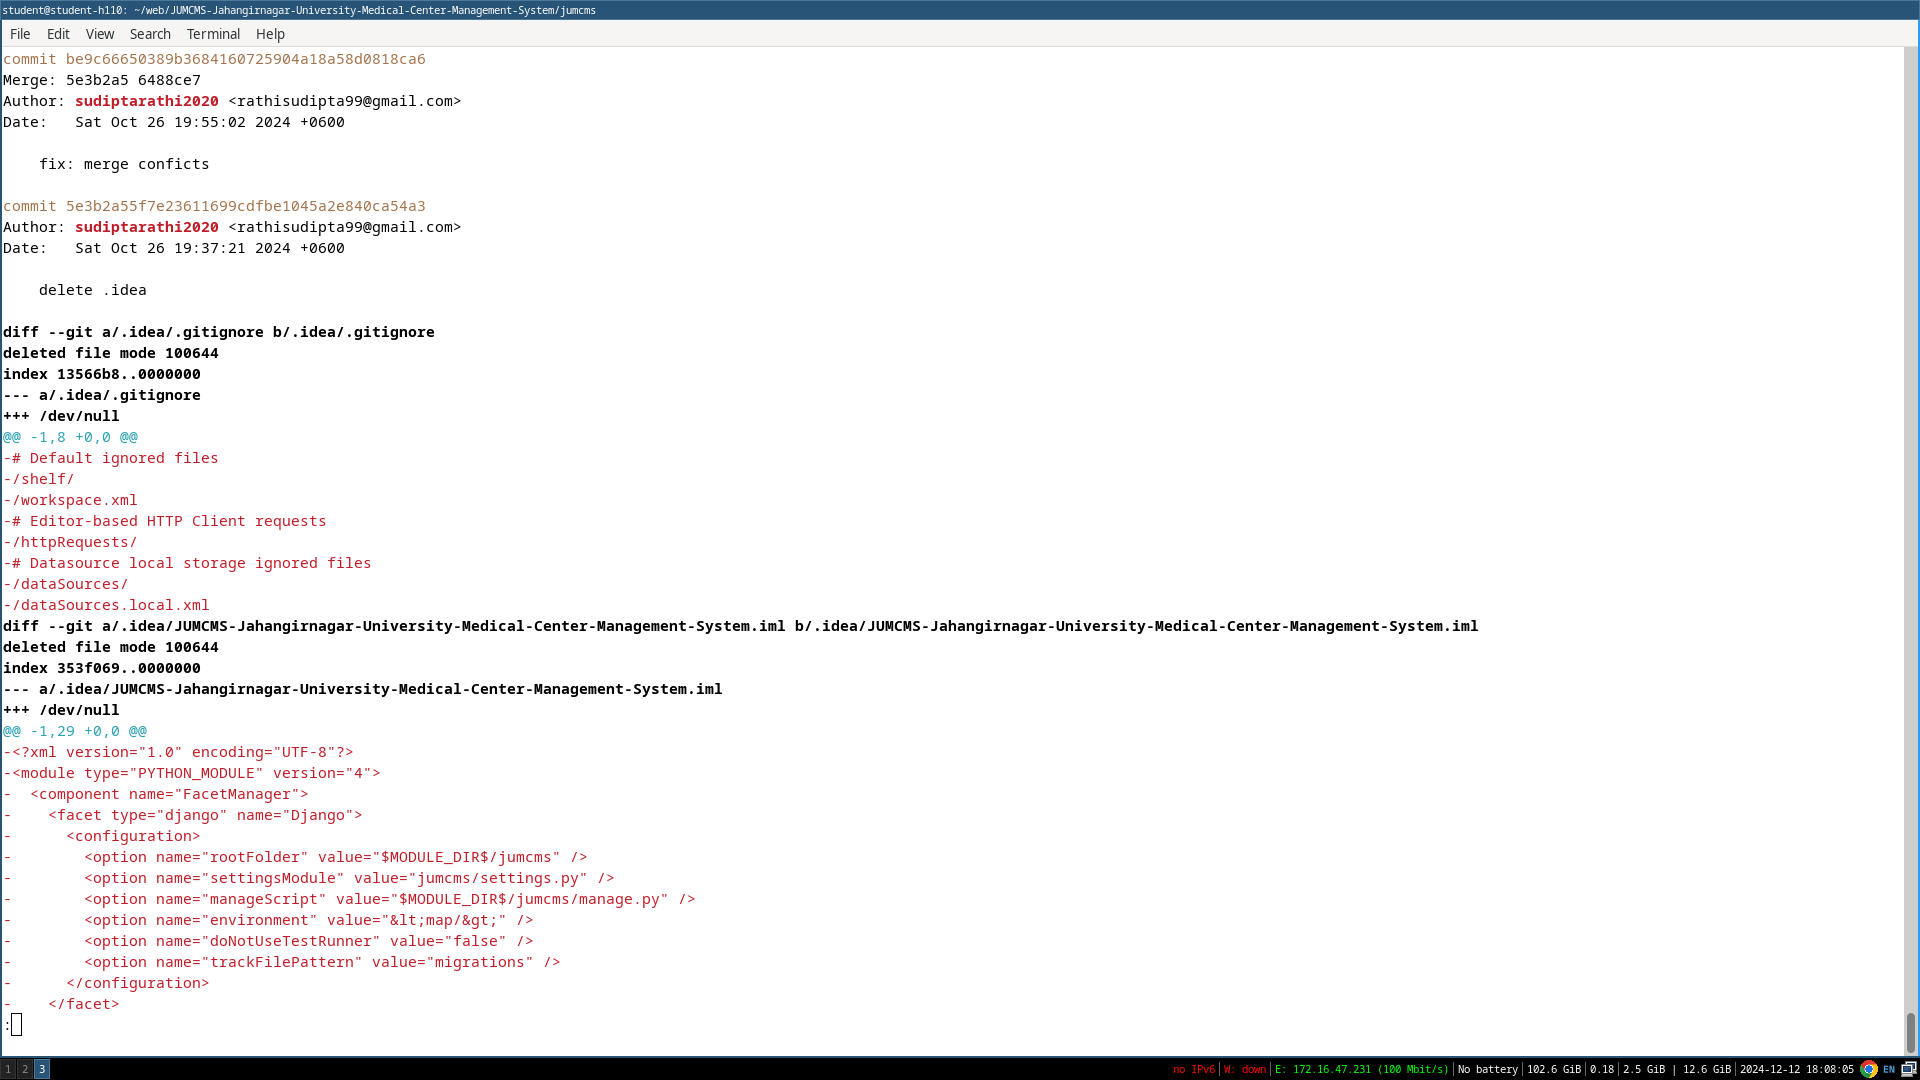
\includegraphics[width=\textwidth]{spr1meet39.png}
    \caption{git message: add dispense medicine logic}
\end{figure}
\newpage
\subsection{Retrospective meeting}
\textbf{What went well:}
\begin{itemize}
    \item Completed Account Creation feature.
    \item Role-based Login functionality was completed successfully where custom tests are passed.
    \item Completed Dispense Medicine feature where custom tests are passed for all feature.
\end{itemize}
\textbf{What could be improved:}
\begin{itemize}
    \item The UI could be improved and more knowledge about URL routing would be helpful for handling challenges in URL routing.
\end{itemize}
\newpage

\section{Unit Testing}
Unit testing is one of the most important task in agile development. After development all the test cases are
passed.
\begin{figure}[H]
    \centering
    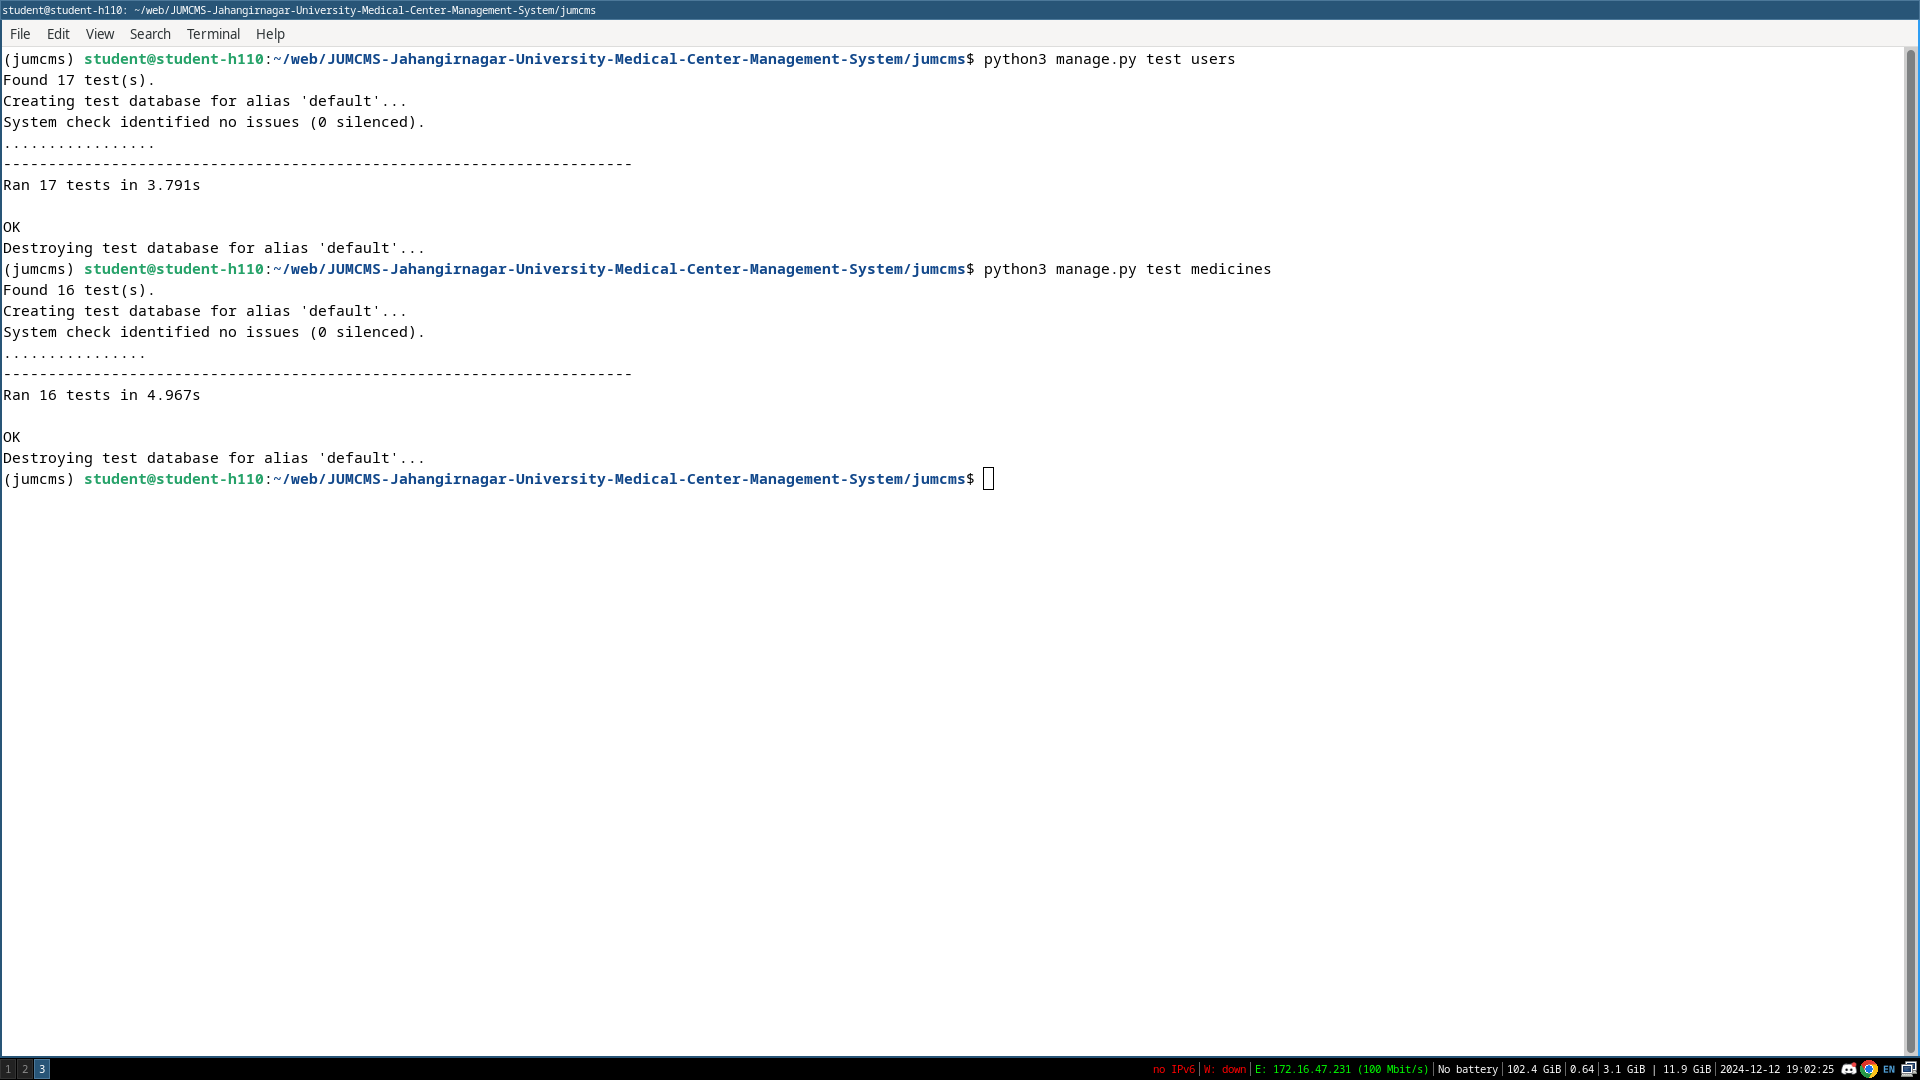
\includegraphics[width=\textwidth]{unittesting.png}
    \caption{Unit Testing Done Successfully}
\end{figure}
\newpage

\section{Working Product after sprint 1}
\begin{figure}[H]
    \centering
    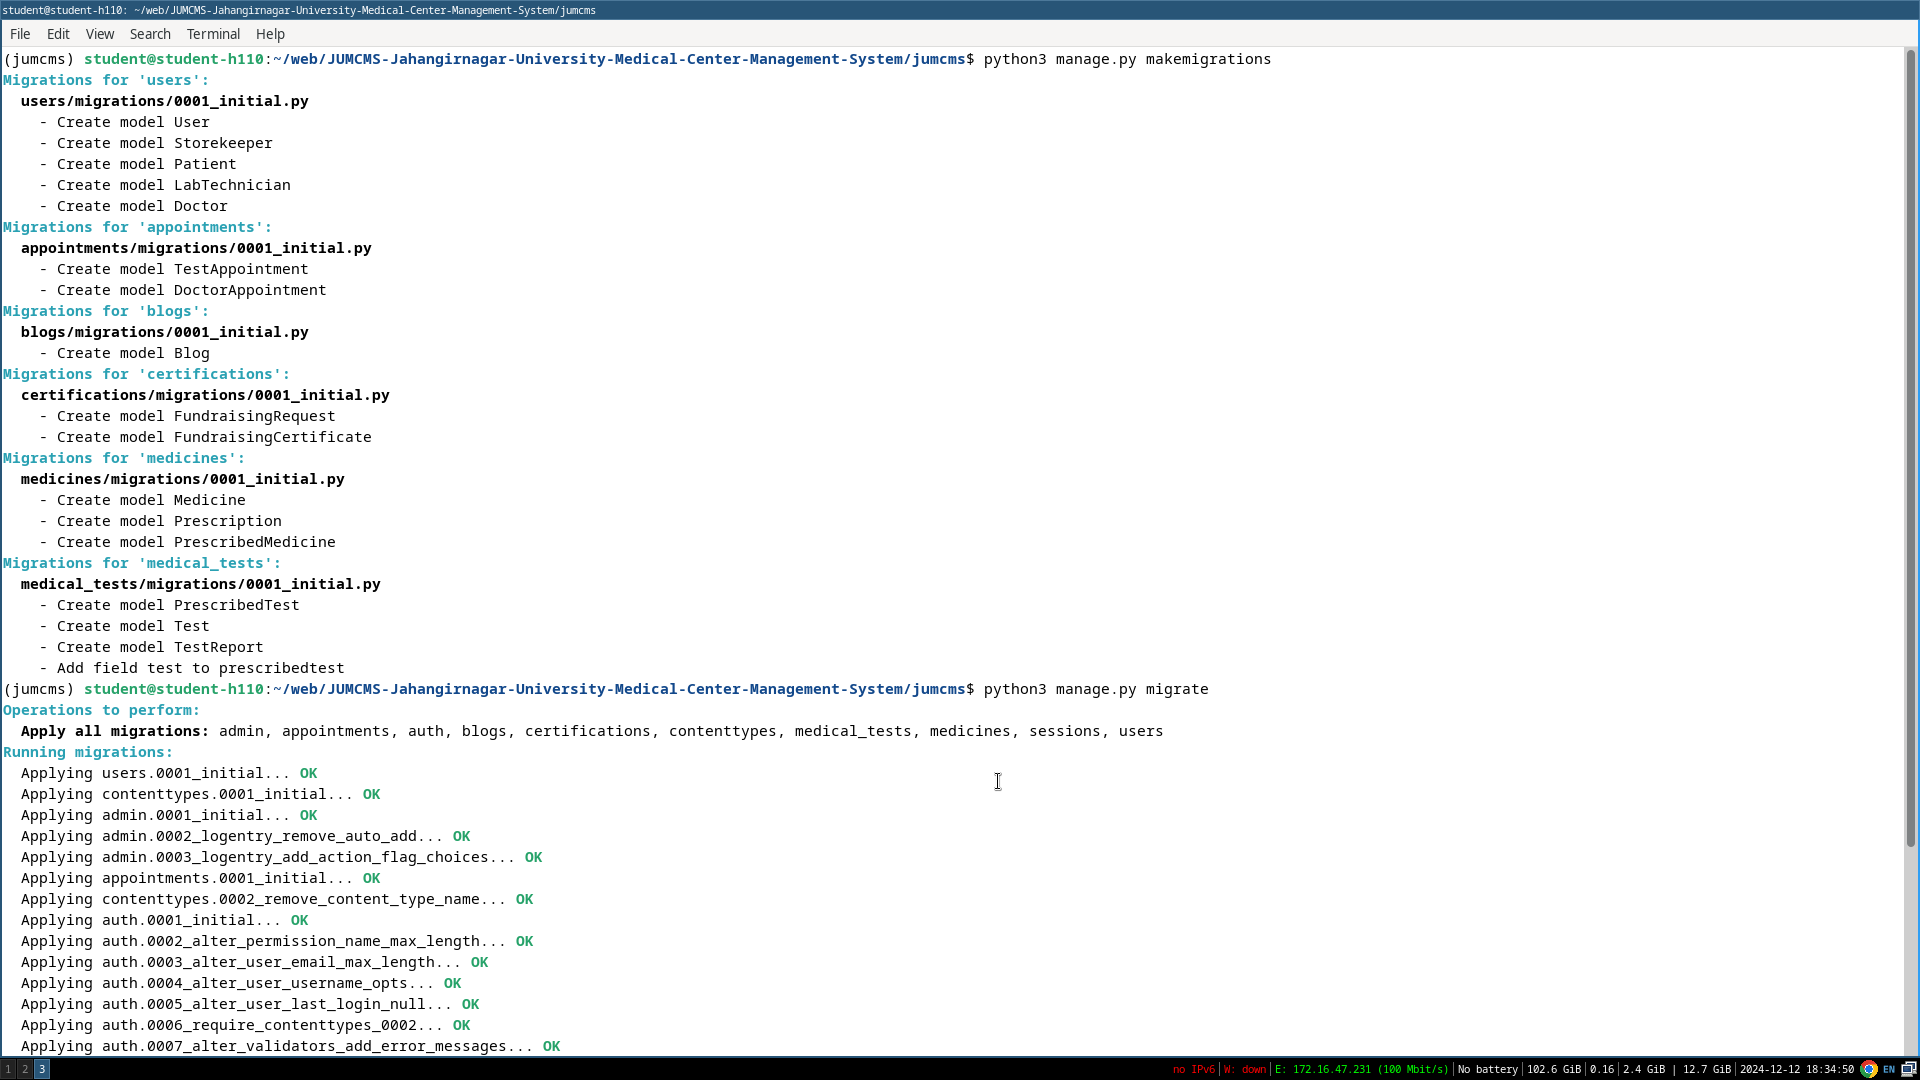
\includegraphics[width=\textwidth]{spr1output1.png}
    \caption{Database migration and migrate}
\end{figure}

\begin{figure}[H]
    \centering
    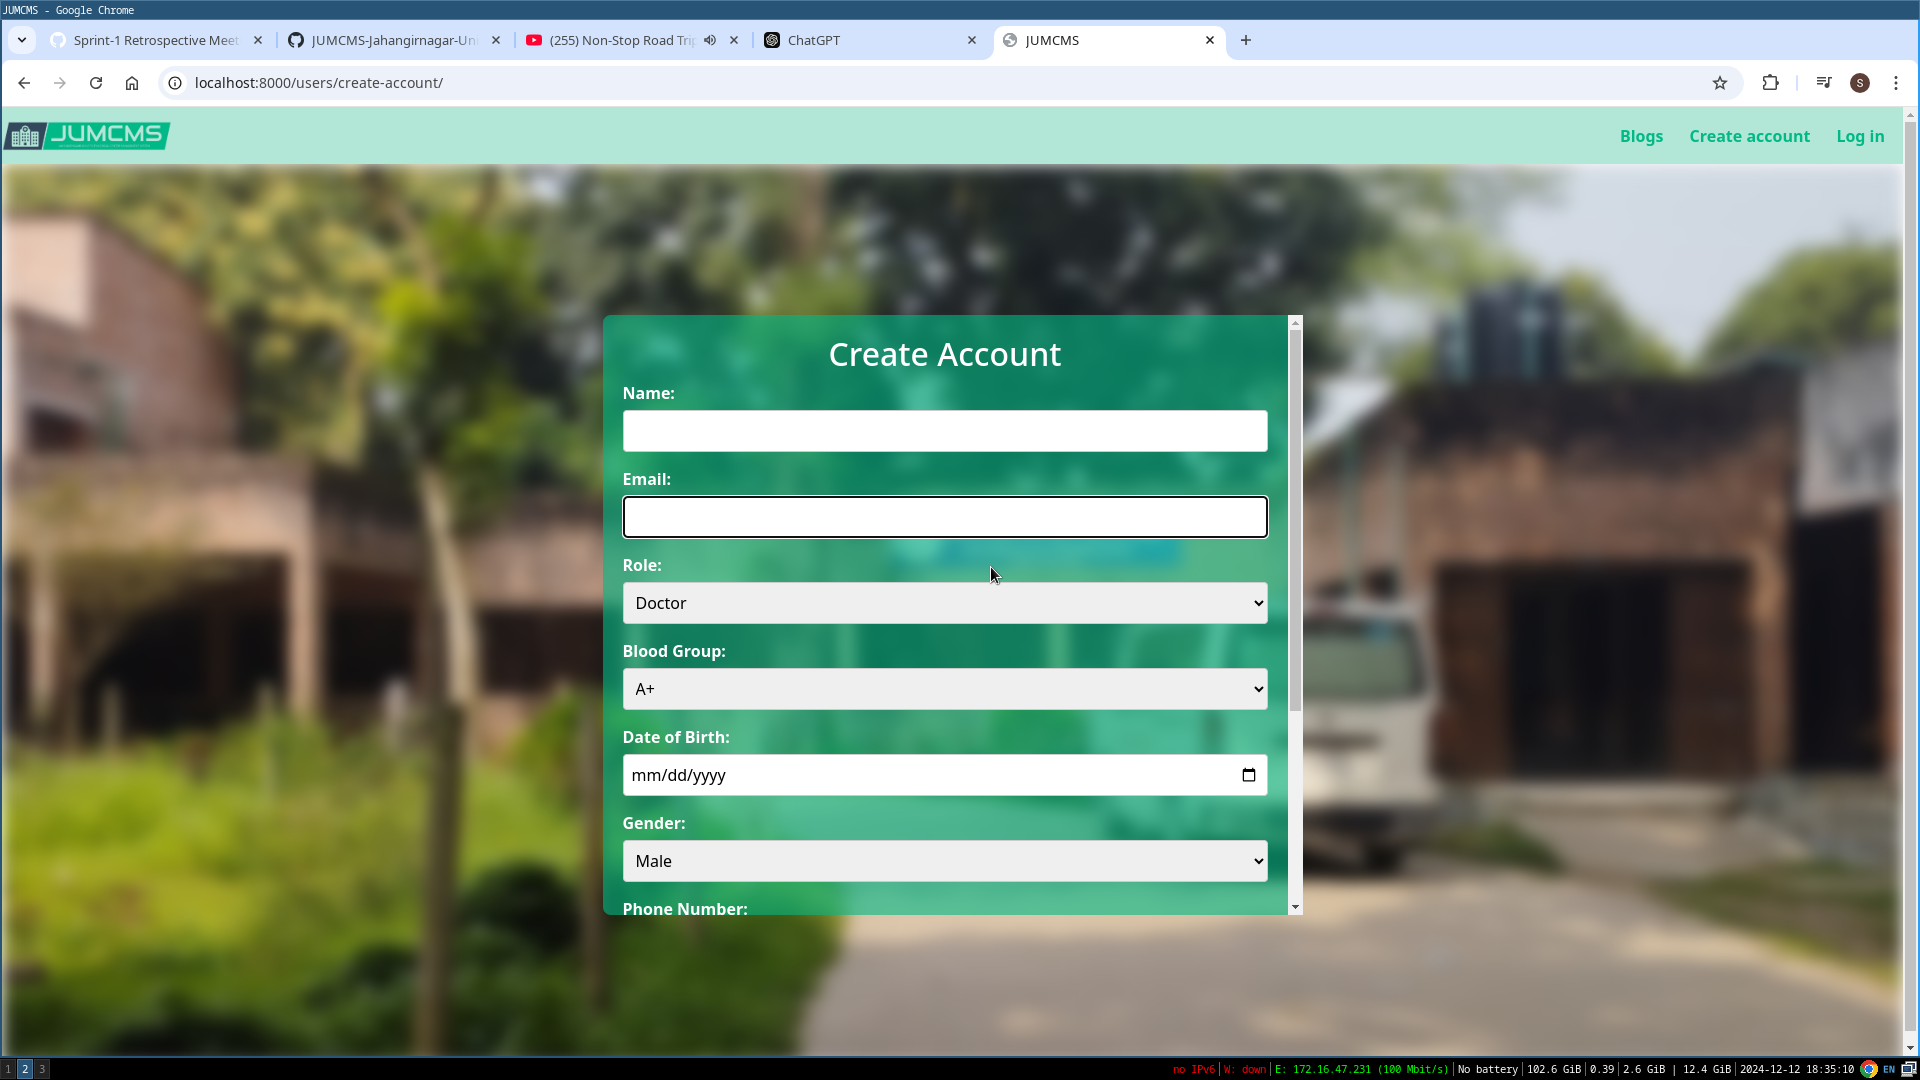
\includegraphics[width=\textwidth]{spr1output2.png}
    \caption{Account Creation Form}
\end{figure}

\begin{figure}[H]
    \centering
    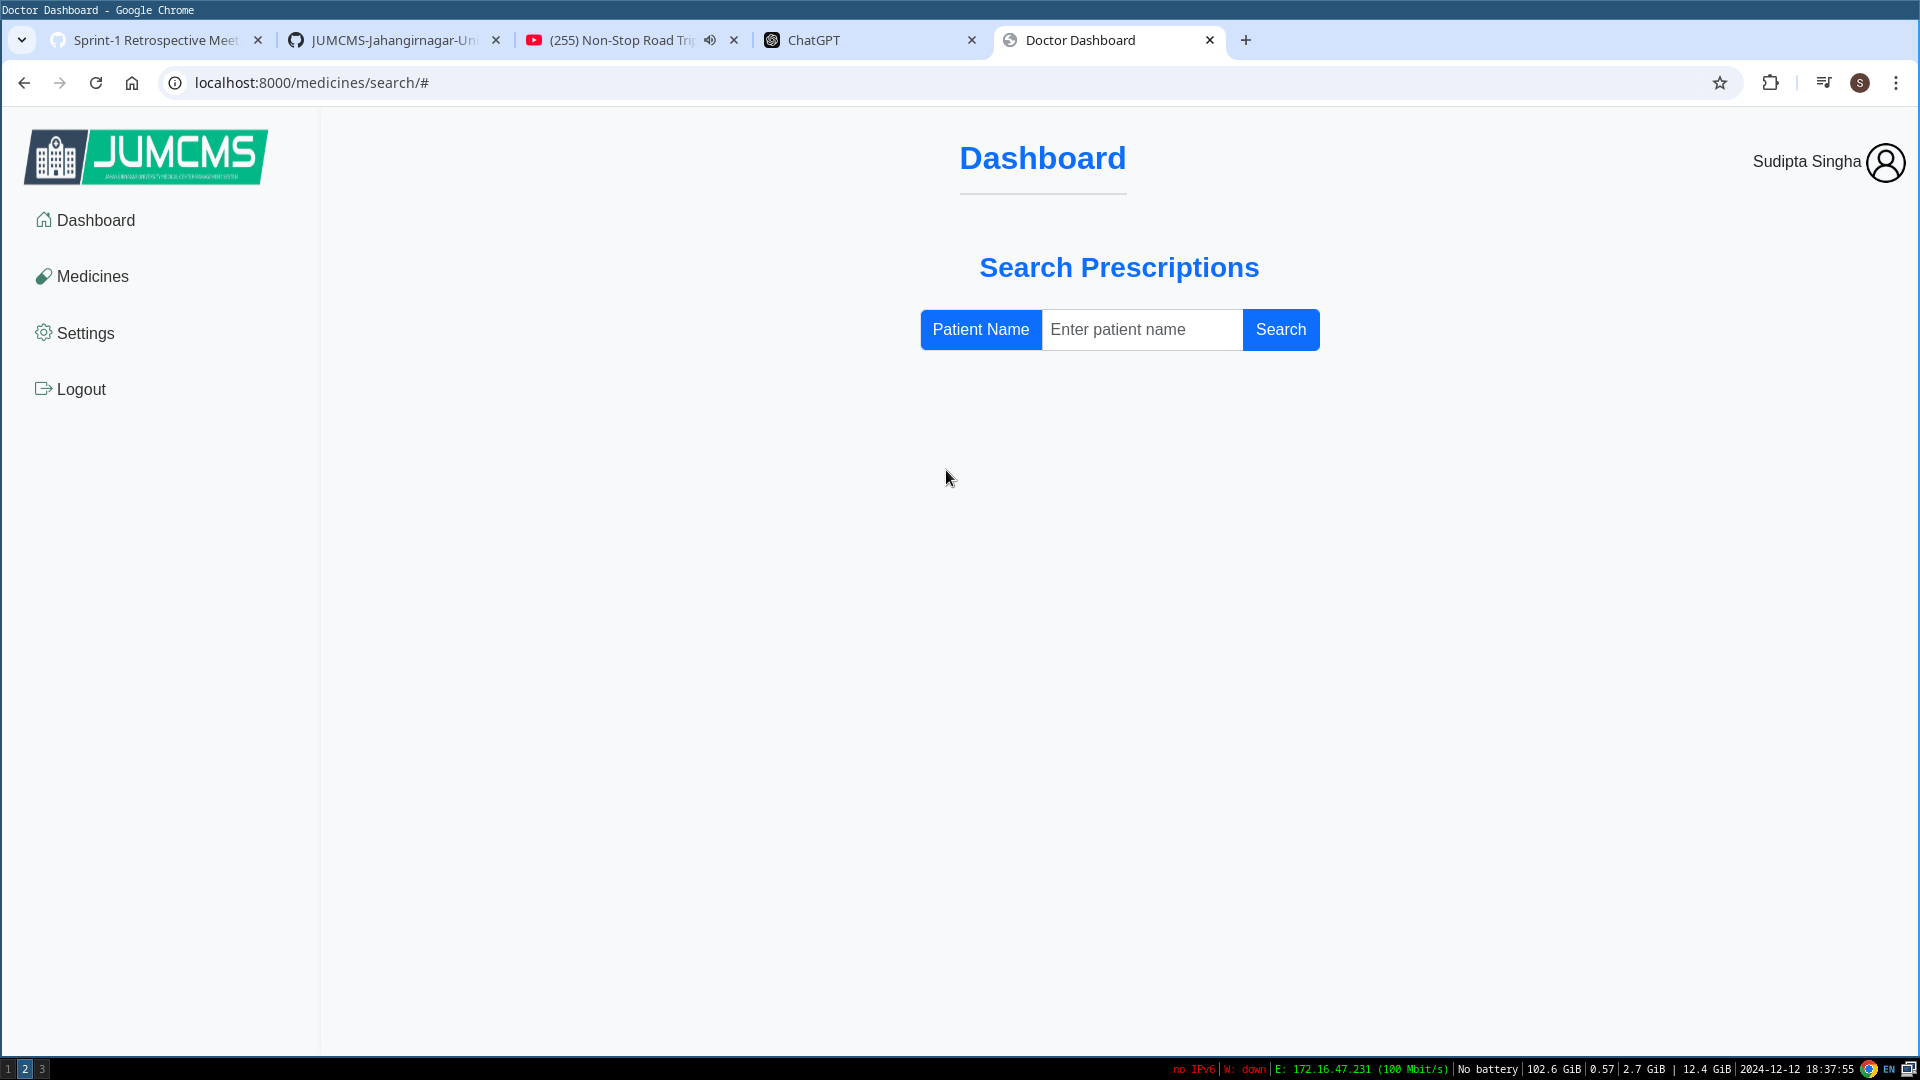
\includegraphics[width=\textwidth]{spr1output3.png}
    \caption{Storekeeper Dashboard}
\end{figure}

\begin{figure}[H]
    \centering
    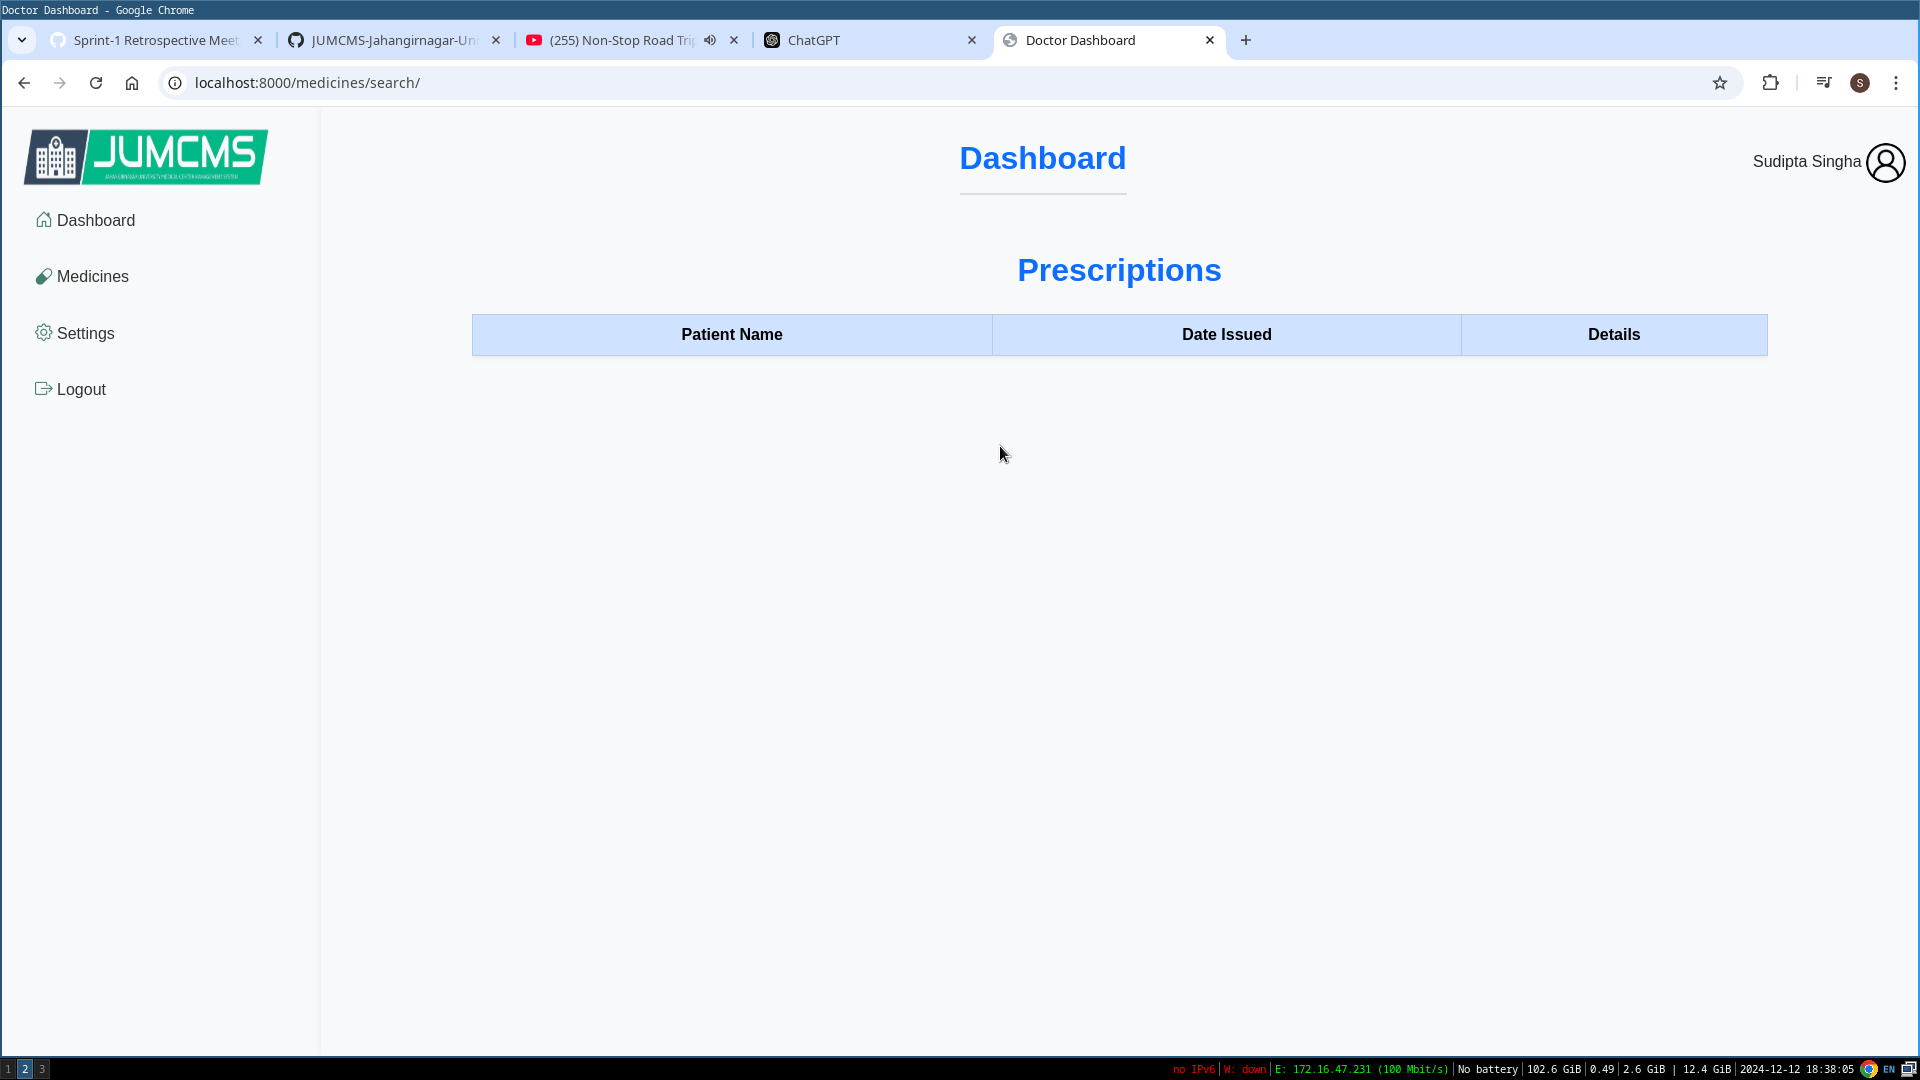
\includegraphics[width=\textwidth]{spr1output4.png}
    \caption{Searching By Patient name}
\end{figure}

\end{document}
